%!Mode:: "TeX:UTF-8"
\documentclass[a4paper,11pt,UTF8]{ctexart}

\usepackage{indentfirst} %缩进
\usepackage{xeCJK}    %使用系统字体
\usepackage{fancyhdr} %自定义页眉页脚
\pagestyle{empty}                   %不设置页眉页脚
\usepackage{amsmath, amsthm, amssymb, amsfonts} %数学公式
\usepackage[a4paper,left=3cm,right=3cm,top=3cm,bottom=3cm]{geometry}
%\usepackage[tmargin=1in,bmargin=1in,lmargin=1.25in,rmargin=1.25in]{geometry}.
\usepackage{booktabs} %插入表格
\usepackage[section]{placeins} %避免浮动
\usepackage{listings} %插入代码
\usepackage{ctex}     %中文宏包
\usepackage[svgnames, table]{xcolor} %彩色表格
\usepackage{algorithm}          %伪代码
\usepackage{algorithmicx}
\usepackage{algpseudocode}
\usepackage{algorithm,algpseudocode,float}
\usepackage{lipsum}
\usepackage{enumitem}           %调整列举环境
\usepackage{url}
\usepackage{fontspec,xunicode}
\defaultfontfeatures{Mapping=tex-text} %如果没有它,会有一些 tex 特殊字符无法正常使用,比如连字符。
\usepackage{subcaption}
\usepackage{graphicx}
\graphicspath{{imgs/}}

%%%%%%%%%%%%%%%%%%%%%%%%%%%%%%%%%%%%%%%%%%%%%%%%%%%%%%%%%%%%%%%%
% 缩进及行间距
%%%%%%%%%%%%%%%%%%%%%%%%%%%%%%%%%%%%%%%%%%%%%%%%%%%%%%%%%%%%%%%%
\setlength{\parindent}{22pt} %重新定义缩进长度
\setlength{\baselineskip}{20pt}  %定义行间距
%\renewcommand{\baselinestretch}{1.1} %定义行间距

%%%%%%%%%%%%%%%%%%%%%%%%%%%%%%%%%%%%%%%%%%%%%%%%%%%%%%%%%%%%%%%%
% 列表设置
%%%%%%%%%%%%%%%%%%%%%%%%%%%%%%%%%%%%%%%%%%%%%%%%%%%%%%%%%%%%%%%%
\setenumerate{fullwidth,itemindent=\parindent,listparindent=\parindent,itemsep=0ex,partopsep=0pt,parsep=0ex}
\setenumerate[2]{label=\alph*),leftmargin=1.5em}  %二级item设置
\setitemize{itemindent=38pt,leftmargin=0pt,itemsep=-0.4ex,listparindent=26pt,partopsep=0pt,parsep=0.5ex,topsep=-0.25ex}
\setdescription{itemindent=38pt,leftmargin=0pt,itemsep=-0.4ex,listparindent=26pt,partopsep=0pt,parsep=0.5ex,topsep=-0.25ex}

%%%%%%%%%%%%%%%%%%%%%%%%%%%%%%%%%%%%%%%%%%%%%%%%%%%%%%%%%%%%%%%%
% 图的标题行间距设置
%%%%%%%%%%%%%%%%%%%%%%%%%%%%%%%%%%%%%%%%%%%%%%%%%%%%%%%%%%%%%%%%
\newcommand{\bottomcaption}{%
\setlength{\abovecaptionskip}{6pt}%
\setlength{\belowcaptionskip}{6pt}%
\caption}


%%%%%%%%%%%%%%%%%%%%%%%%%%%%%%%%%%%%%%%%%%%%%%%%%%%%%%%%%%%%%%%%
% 字体定义
%%%%%%%%%%%%%%%%%%%%%%%%%%%%%%%%%%%%%%%%%%%%%%%%%%%%%%%%%%%%%%%%
\setmainfont{Times New Roman}  %默认英文字体.serif是有衬线字体sans serif无衬线字体
\setmonofont{Consolas}
\setCJKmainfont[ItalicFont={楷体}, BoldFont={黑体}]{宋体}%衬线字体 缺省中文字体为
\setCJKsansfont{黑体}
\punctstyle{hangmobanjiao}
%-----------------------xeCJK下设置中文字体------------------------------%
\setCJKfamilyfont{song}{SimSun}                             %宋体 song
\newcommand{\song}{\CJKfamily{song}}
\setCJKfamilyfont{fs}{FangSong}                      %仿宋  fs
\newcommand{\fs}{\CJKfamily{fs}}
\setCJKfamilyfont{ktgb}{KaiTi}                      %楷体2312 ktgb
\newcommand{\ktgb}{\CJKfamily{ktgb}}
\setCJKfamilyfont{yh}{Microsoft YaHei}                    %微软雅黑 yh
\newcommand{\yh}{\CJKfamily{yh}}
\setCJKfamilyfont{hei}{SimHei}                              %黑体  hei
\newcommand{\hei}{\CJKfamily{hei}}
\setCJKfamilyfont{hwxk}{STXingkai}                                %华文行楷  hwxk
\newcommand{\hwxk}{\CJKfamily{hwxk}}
%------------------------------设置字体大小------------------------%
\newcommand{\shiyanbaogao}{\fontsize{36pt}{\baselineskip}\selectfont}
\newcommand{\chuhao}{\fontsize{42pt}{\baselineskip}\selectfont}     %初号
\newcommand{\xiaochuhao}{\fontsize{36pt}{\baselineskip}\selectfont} %小初号
\newcommand{\yihao}{\fontsize{28pt}{\baselineskip}\selectfont}      %一号
\newcommand{\erhao}{\fontsize{21pt}{\baselineskip}\selectfont}      %二号
\newcommand{\xiaoerhao}{\fontsize{18pt}{\baselineskip}\selectfont}  %小二号
\newcommand{\sanhao}{\fontsize{15.75pt}{\baselineskip}\selectfont}  %三号
\newcommand{\sihao}{\fontsize{14pt}{\baselineskip}\selectfont}       %四号
\newcommand{\xiaosihao}{\fontsize{12pt}{\baselineskip}\selectfont}  %小四号
\newcommand{\wuhao}{\fontsize{10.5pt}{\baselineskip}\selectfont}    %五号
\newcommand{\xiaowuhao}{\fontsize{9pt}{\baselineskip}\selectfont}   %小五号
\newcommand{\liuhao}{\fontsize{7.875pt}{\baselineskip}\selectfont}  %六号
\newcommand{\qihao}{\fontsize{5.25pt}{\baselineskip}\selectfont}    %七号

%%%%%%%%%%%%%%%%%%%%%%%%%%%%%%%%%%%%%%%%%%%%%%%%%%%%%%%%%%%%%%%%
% 图题字体大小相同
%%%%%%%%%%%%%%%%%%%%%%%%%%%%%%%%%%%%%%%%%%%%%%%%%%%%%%%%%%%%%%%%
\usepackage{caption}
\captionsetup{font={footnotesize}}   % footnotesize = 9pt
\captionsetup[lstlisting]{font={footnotesize}}

%%%%%%%%%%%%%%%%%%%%%%%%%%%%%%%%%%%%%%%%%%%%%%%%%%%%%%%%%%%%%%%%
% 重定义枚举编号为 1),2)...
%%%%%%%%%%%%%%%%%%%%%%%%%%%%%%%%%%%%%%%%%%%%%%%%%%%%%%%%%%%%%%%%
\renewcommand{\labelenumi}{\theenumi}


%%%%%%%%%%%%%%%%%%%%%%%%%%%%%%%%%%%%%%%%%%%%%%%%%%%%%%%%%%%%%%%%
% 重定义section标题
%%%%%%%%%%%%%%%%%%%%%%%%%%%%%%%%%%%%%%%%%%%%%%%%%%%%%%%%%%%%%%%%
\CTEXsetup[format={\sihao\CJKfamily{zhhei}\zihao{4}},number={\chinese{section}},name={,、~},aftername={},indent={0pt},beforeskip={6pt},afterskip={6pt},format+={\flushleft}]{section}
\CTEXsetup[number={\chinese{section}},name={附录, ~~ }]{appendix}



%%%%%%%%%%%%%%%%%%%%%%%%%%%%%%%%%%%%%%%%%%%%%%%%%%%%%%%%%%%%%%%%
% 标题名称中文化
%%%%%%%%%%%%%%%%%%%%%%%%%%%%%%%%%%%%%%%%%%%%%%%%%%%%%%%%%%%%%%%%
\renewcommand\figurename{\hei 图}
\renewcommand\tablename{\hei 表}
\renewcommand\lstlistingname{\hei 代码}
\renewcommand{\algorithmicrequire}{\textbf{输入:}}
\renewcommand{\algorithmicensure}{\textbf{输出:}}
\newtheorem{define}{定义}

%%%%%%%%%%%%%%%%%%%%%%%%%%%%%%%%%%%%%%%%%%%%%%%%%%%%%%%%%%%%%%%%
% 代码设置
%%%%%%%%%%%%%%%%%%%%%%%%%%%%%%%%%%%%%%%%%%%%%%%%%%%%%%%%%%%%%%%%
\lstset{
 columns=fixed,
 numbers=left,                                        % 在左侧显示行号
 numberstyle=\tiny\color{gray},                       % 设定行号格式
 frame=single,                                        % 单线背景边框
 breaklines=true,                                     % 设定LaTeX对过长的代码行进行自动换行
 keywordstyle=\color[RGB]{40,40,255},                 % 设定关键字颜色
 numberstyle=\footnotesize\color{darkgray},
 commentstyle=\it\color[RGB]{0,96,96},                % 设置代码注释的格式
 stringstyle=\rmfamily\slshape\color[RGB]{128,0,0},   % 设置字符串格式
 showstringspaces=false,                              % 不显示字符串中的空格
 language=java,                                        % 设置语言
 basicstyle=\linespread{1.0}\xiaowuhao\ttfamily,                      % 字体字号
 %lineskip=10pt,
 %baselinestretch=1,
}

%%%%%%%%%%%%%%%%%%%%%%%%%%%%%%%%%%%%%%%%%%%%%%%%%%%%%%%%%%%%%%%%
% 伪代码分页
%%%%%%%%%%%%%%%%%%%%%%%%%%%%%%%%%%%%%%%%%%%%%%%%%%%%%%%%%%%%%%%%
\makeatletter
\renewcommand{\ALG@name}{算法}
\newenvironment{breakablealgorithm}
  {% \begin{breakablealgorithm}
   \begin{center}
     \refstepcounter{algorithm}% New algorithm
     \hrule height.8pt depth0pt \kern2pt% \@fs@pre for \@fs@ruled
     \renewcommand{\caption}[2][\relax]{% Make a new \caption
       {\raggedright\textbf{\ALG@name~\thealgorithm} ##2\par}%
       \ifx\relax##1\relax % #1 is \relax
         \addcontentsline{loa}{algorithm}{\protect\numberline{\thealgorithm}##2}%
       \else % #1 is not \relax
         \addcontentsline{loa}{algorithm}{\protect\numberline{\thealgorithm}##1}%
       \fi
       \kern2pt\hrule\kern2pt
     }
  }{% \end{breakablealgorithm}
     \kern2pt\hrule\relax% \@fs@post for \@fs@ruled
   \end{center}
  }
\makeatother



\begin{document}
\xiaosihao\song

\begin{titlepage}
\center{\yihao{\hwxk{武汉大学国家网络安全学院}}}
\vspace{6cm}
\center{\shiyanbaogao{\ktgb{密~码~学~实~验~报~告}}}
\vspace{4cm}

\begin{center}
\begin{large}
\begin{tabular}{rc}
\xiaoerhao{\hei{学\qquad 号}}& \hspace{1.7cm}\xiaoerhao{\hei{2021302181156\hspace{1.7cm}}} \\
\cline{2-2}\\
\xiaoerhao{\hei{姓\qquad 名}}& \xiaoerhao{\hei{赵~伯~俣}}\\
\cline{2-2}\\
\xiaoerhao{\hei{实验名称}}& \xiaoerhao{\hei{分组密码DES}}\\
\cline{2-2}\\
\xiaoerhao{\hei{指导教师}}& \xiaoerhao{\hei{何琨}}\\
\cline{2-2}
\end{tabular}
\end{large}
\end{center}
\vfill \hfill
\end{titlepage}
\clearpage

% \centerline{\\[10pt]\erhao{\fs{武 ~汉 ~ 大~ 学}}}
% \centerline{\\[10pt]\yihao{\fs{信~息~隐~藏~实~验~报~告}}}

% \leftline{\\[10pt]\sihao{\hei{\hspace{1.5em} 学生姓名:XXX \hfill 学号:XXXX \hfill 指导教师:XXX }}}

% \leftline{\\[10pt]\sihao{\hei{\hspace{1.5em} 实验地点:新珈楼XXX \hfill }}}

% \leftline{\\[10pt]\sihao{\hei{\hspace{1.5em} 实验时间:第X周周X(X-X节) \hfill }}}



\setlength{\parskip}{6pt}  %定义段间距

\section{实验名称: 分组密码DES}
\section{实验目的及要求:}
    \subsection{实验目的}
        $(1)$掌握分组密码的基本概念;\par
        $(2)$掌握DES(3DES)密码算法;\par
        $(3)$了解DES(3DES)密码的安全性;\par
        $(4)$掌握分组密码常用工作模式及其特点;\par
        $(5)$熟悉分组密码的应用。
    \subsection{实验要求}
        $(1)$复习掌握(古典密码)使用的置换、代替、XOR、迭代等技术;\par
        $(2)$比较DES中代替技术与古典密码中的联系与区别;\par
        $(3)$理解S盒、P置换等部件的安全性准则;\par
        $(4)$实现DES算法的编程与优化。\par


\section{实验设备环境及要求:}
    Windows操作系统,python高级语言开发环境
\newpage
\section{实验内容与步骤:}
    \subsection{DES 子密钥扩展算法的实现}
        子密钥拓展算法是将64位密钥经过置换选择1、循环左移、置换选择2等变换,
        产出16个48位长的子密钥,子密钥的产生过程如下图所示
        \begin{figure}[H]
            \centering
            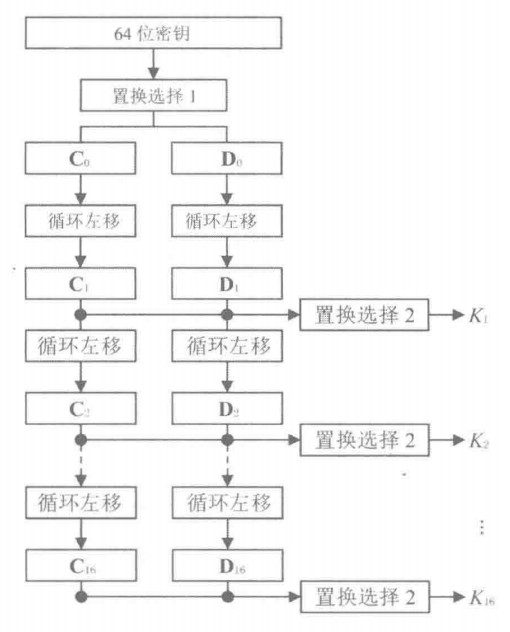
\includegraphics[width=9cm]{get_keys.png}
            \bottomcaption{\xiaowuhao{子密钥的产生}}
        \end{figure}
        其中子密钥的生成总体算法如下所示
        \lstinputlisting[caption={子密钥生成代码},captionpos=b,firstline=47, lastline=73]{E:/Python_code/codes/密码学/lab_1/KEY.py}
\newpage
        \subsubsection{置换选择1}
            置换选择1的作用一是为了从64位密钥中去掉8个奇偶校验位;二是为了把其余的56位密钥位打乱顺序
            重新排列,并且将前28位作为C0,后28位作为D0,其中置乱选择1使用的置换矩阵如下图所示
            \begin{figure}[H]
                \centering
                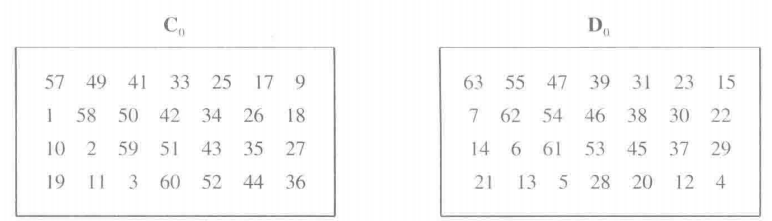
\includegraphics[width=9cm]{PC_1.png}
                \bottomcaption{\xiaowuhao{置换选择1矩阵}}
            \end{figure}
            该步骤的代码如下所示
            \lstinputlisting[caption={置换选择1代码},captionpos=b,firstline=1, lastline=11]{E:/Python_code/codes/密码学/lab_1/place_change.py}
\newpage
        \subsubsection{循环左移}
            循环左移是在每一轮次的子密钥生成过程中对$c_{n-1}$和$d_{n-1}$按照循环左移位数表中的值进行循环左移,
            得到$c_{n}$和$d_{n}$,n为当前轮次。循环左移位数表如下图所示
            \begin{figure}[H]
                \centering
                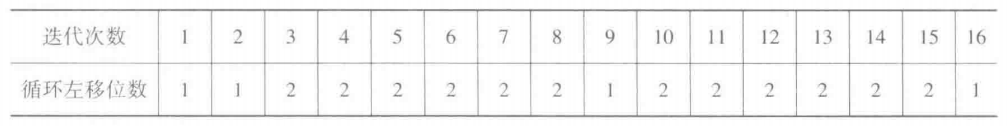
\includegraphics[width=9cm]{left_shift.png}
                \bottomcaption{\xiaowuhao{循环左移位数表}}
            \end{figure}
            该步骤的代码如下图所示
            \lstinputlisting[caption={循环左移代码},captionpos=b,firstline=38, lastline=44]{E:/Python_code/codes/密码学/lab_1/KEY.py}
\newpage
        \subsubsection{置换选择2}
            置乱选择2是将$c_{n}$和$d_{n}$合并成一个56位的中间数据后按照置乱选择2矩阵从中选择出一个48位的子密钥$K_{n}$,
            置乱选择2的矩阵如下图所示
            \begin{figure}[H]
                \centering
                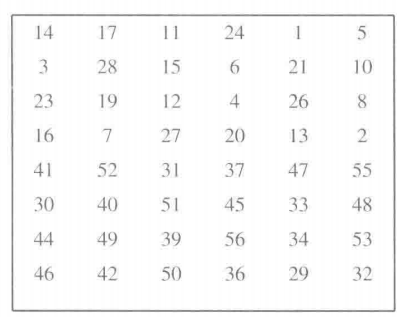
\includegraphics[width=6cm]{PC_2.png}
                \bottomcaption{\xiaowuhao{置乱选择2矩阵}}
            \end{figure}
            该步骤的代码如下所示
            \lstinputlisting[caption={置换选择2代码},captionpos=b,firstline=14, lastline=28]{E:/Python_code/codes/密码学/lab_1/place_change.py}

    \subsection{DES局部加密函数f的实现}
        局部加密函数的作用是在第i次加密迭代中用子密钥$k_{i}$对$R_{i-1}$进行加密,首先进行选择运算E对32位的$R_{i-1}$的各位进行选择和排列,产生一个48位的结果,
        然后将得到的结果与子密钥$k_{i}$进行异或操作,然后送入整体S盒中,产生32位的数据组,经过置换运算P将各位打乱重拍后得到加密函数的密文输出\par
        该加密函数f算法流程图如下图所示    
        \begin{figure}[H]
            \centering
            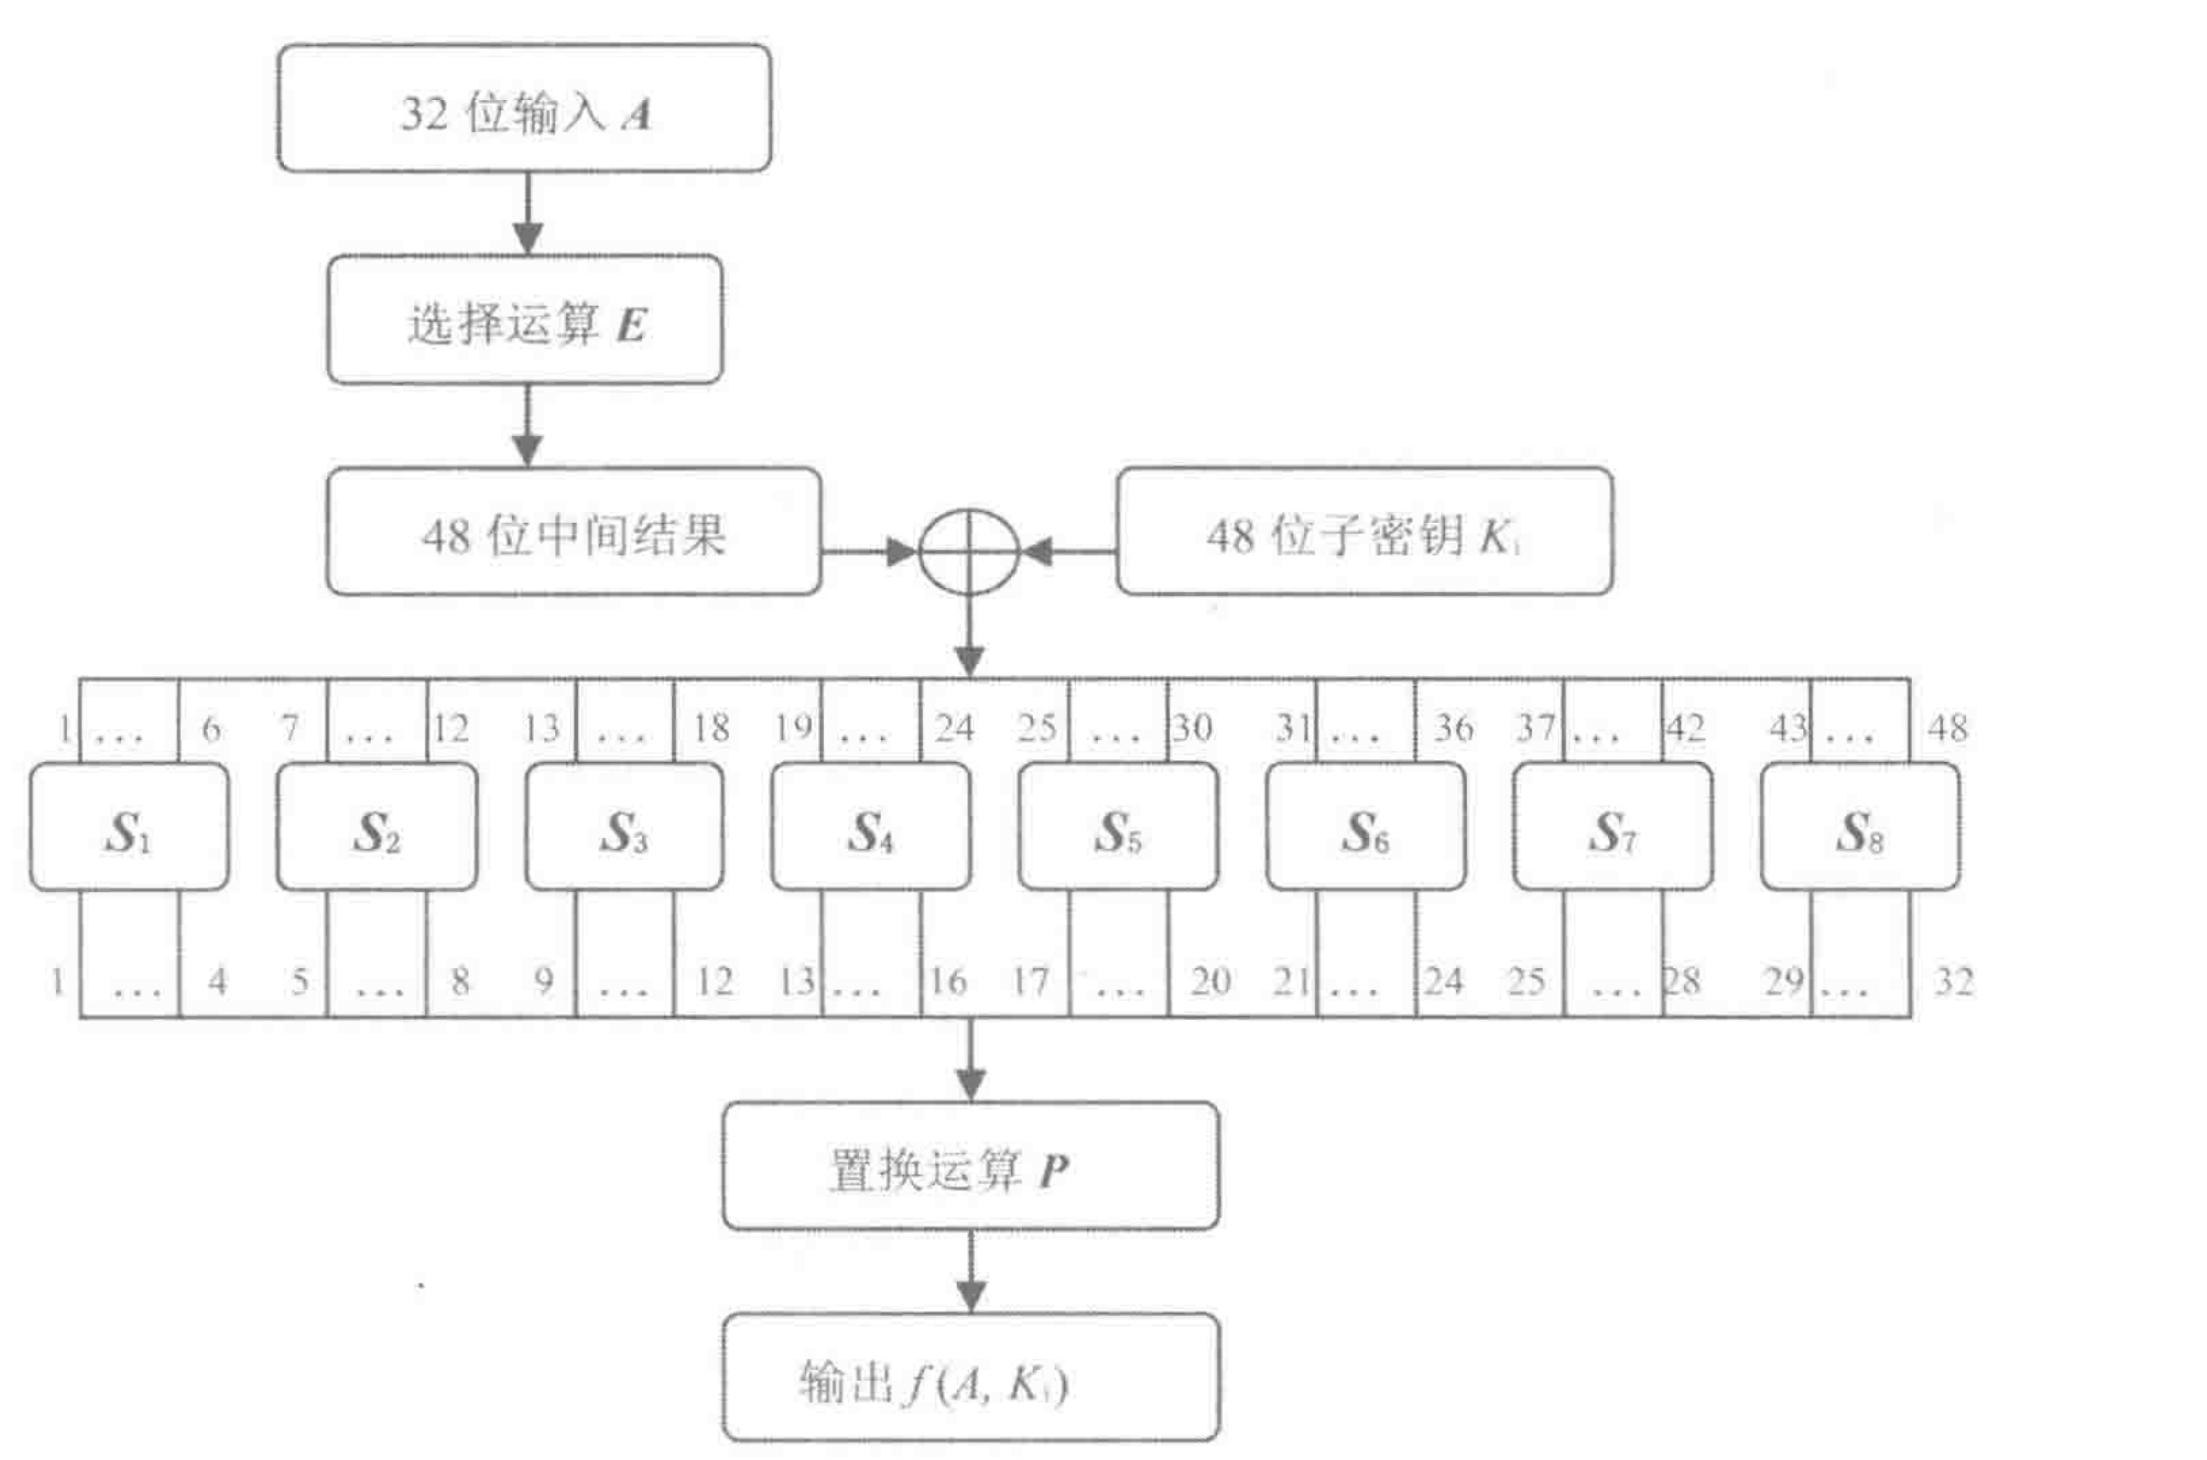
\includegraphics[width=9cm]{f.jpg}
            \bottomcaption{\xiaowuhao{加密函数f}}
        \end{figure}
        该加密函数的代码如下所示
        \lstinputlisting[caption={加密函数f代码},captionpos=b,firstline=70, lastline=80]{E:/Python_code/codes/密码学/lab_1/F.py}

        \subsubsection{扩展置换E}
            选择运算E对32位的数据A的各位进行重复选择某些数据产生一个48位的结果,以达到数据拓展的目的,其中选择运算E的矩阵如下图所示
            \begin{figure}[H]
                \centering
                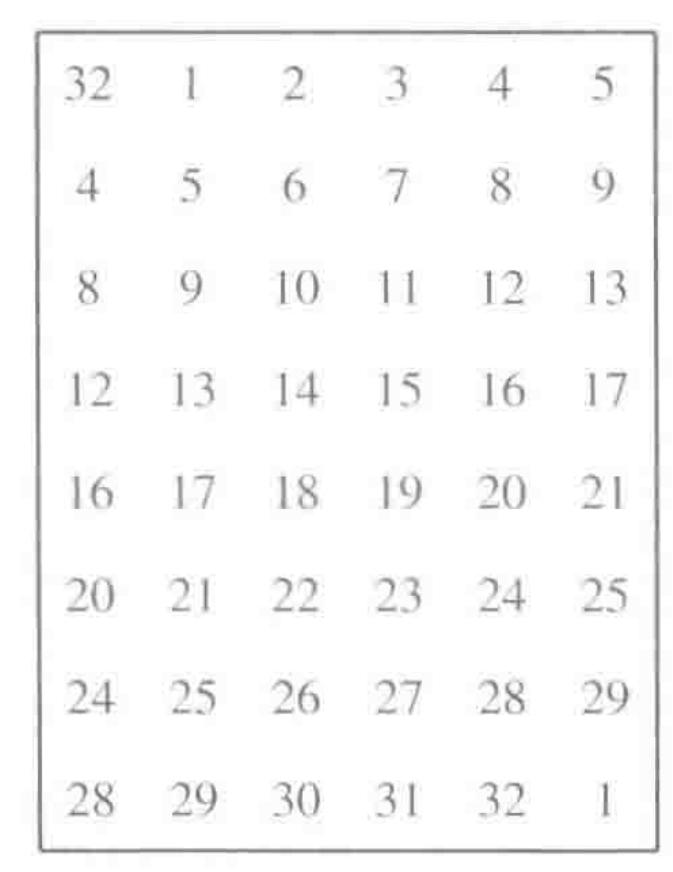
\includegraphics[width=6cm]{E.jpg}
                \bottomcaption{\xiaowuhao{拓展置换矩阵}}
            \end{figure}
            进行拓展置换的程序代码如下所示
            \lstinputlisting[caption={拓展置换函数E代码},captionpos=b,firstline=38, lastline=44]{E:/Python_code/codes/密码学/lab_1/place_change.py}

        \subsubsection{异或操作}
            异或操作是针对输入的两个矩阵的每一位进行异或操作后输出,其程序代码如下所示
            \lstinputlisting[caption={异或操作代码},captionpos=b,firstline=8, lastline=13]{E:/Python_code/codes/密码学/lab_1/F.py}
        \subsubsection{代替S盒}
            代替S盒由8个S盒组成,对于每一个S盒有6位输入,产生4位的输出,因此整体的S盒接收48位输入数据,返回32位的输出,
            在一个单个的S盒中,将6位输入的首尾两位作为选中的行号,将中间4位作为列号,在当前的S盒矩阵中进行查找,将查找到的
            结果以4位2进制的形式进行输出。
            S盒的代替矩阵如下图所示
            \begin{figure}[H]
                \centering 
                \begin{subfigure}[b]{0.4\textwidth}
                    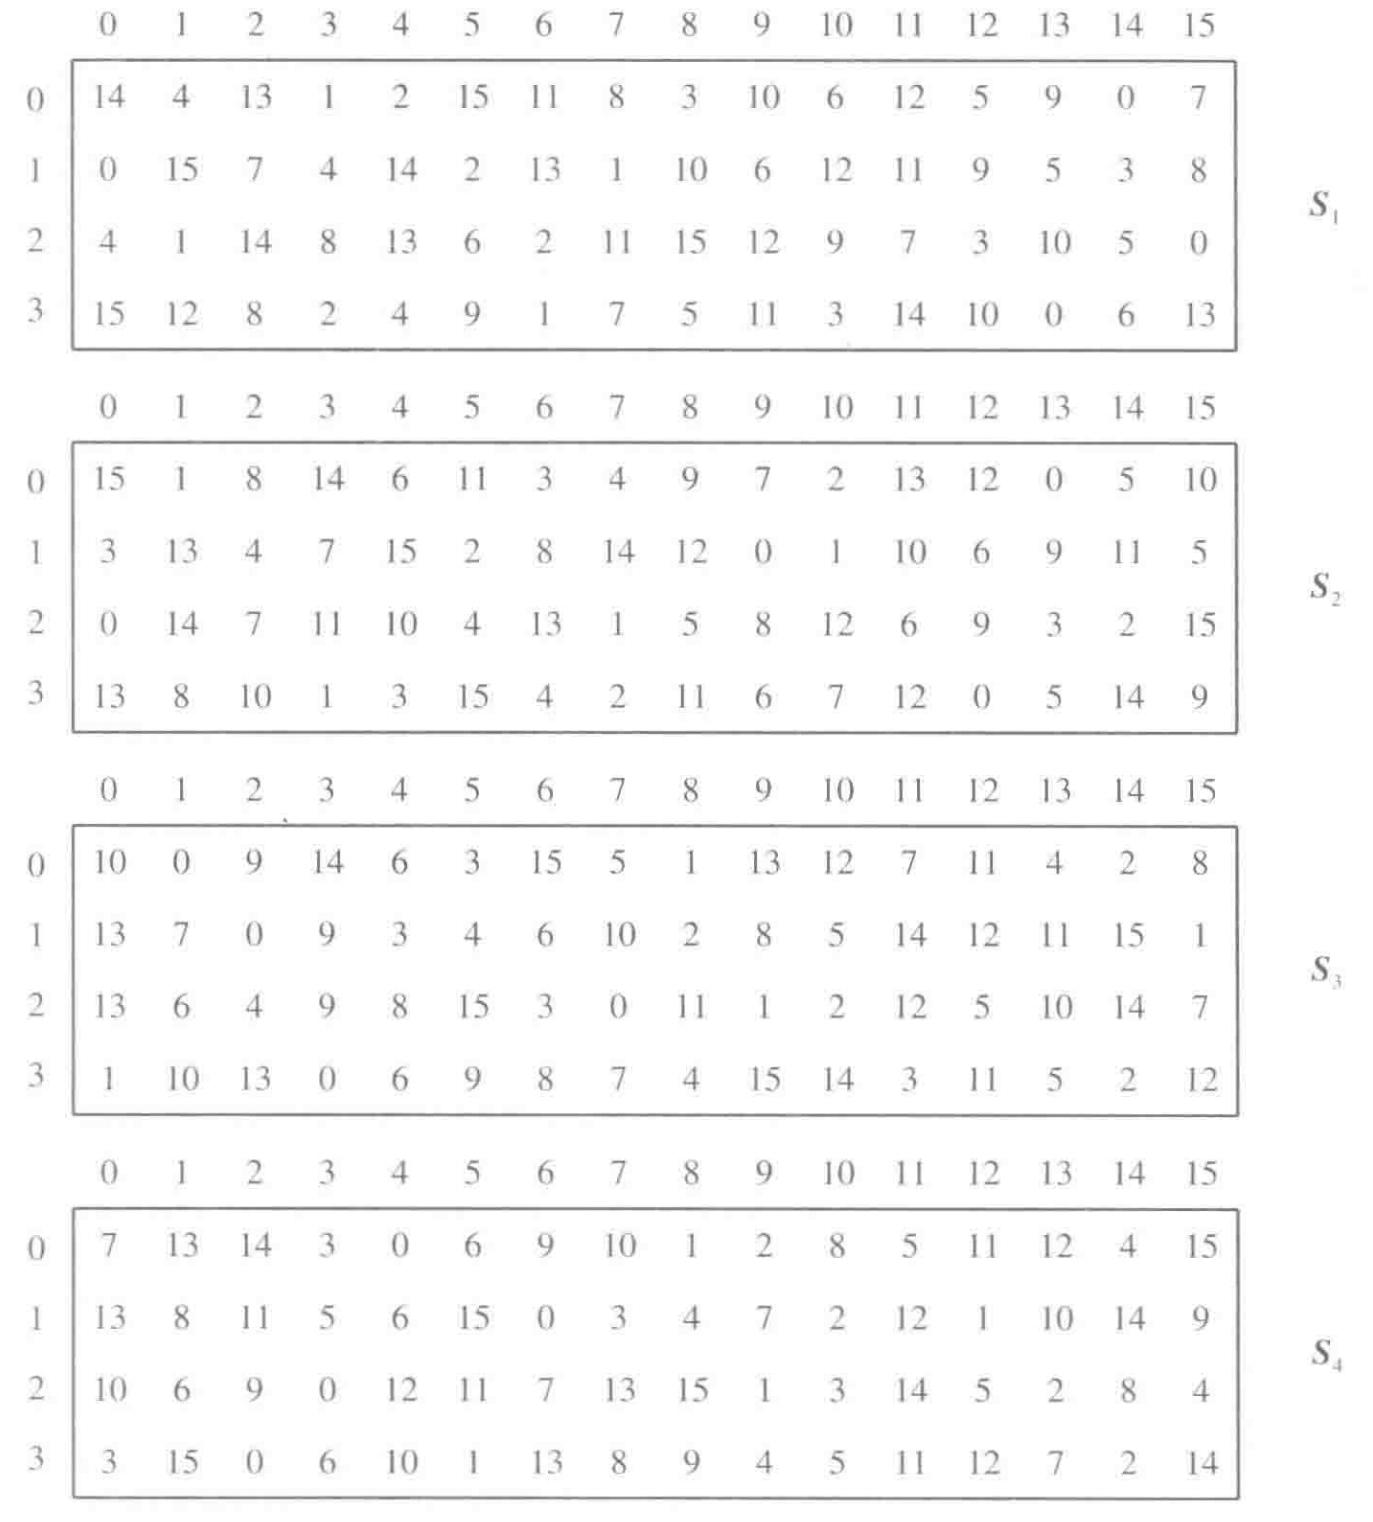
\includegraphics[width=\textwidth]{S_1.jpg}
                    \label{fig:subfig1}
                \end{subfigure}
                \hfill
                \begin{subfigure}[b]{0.4\textwidth}
                    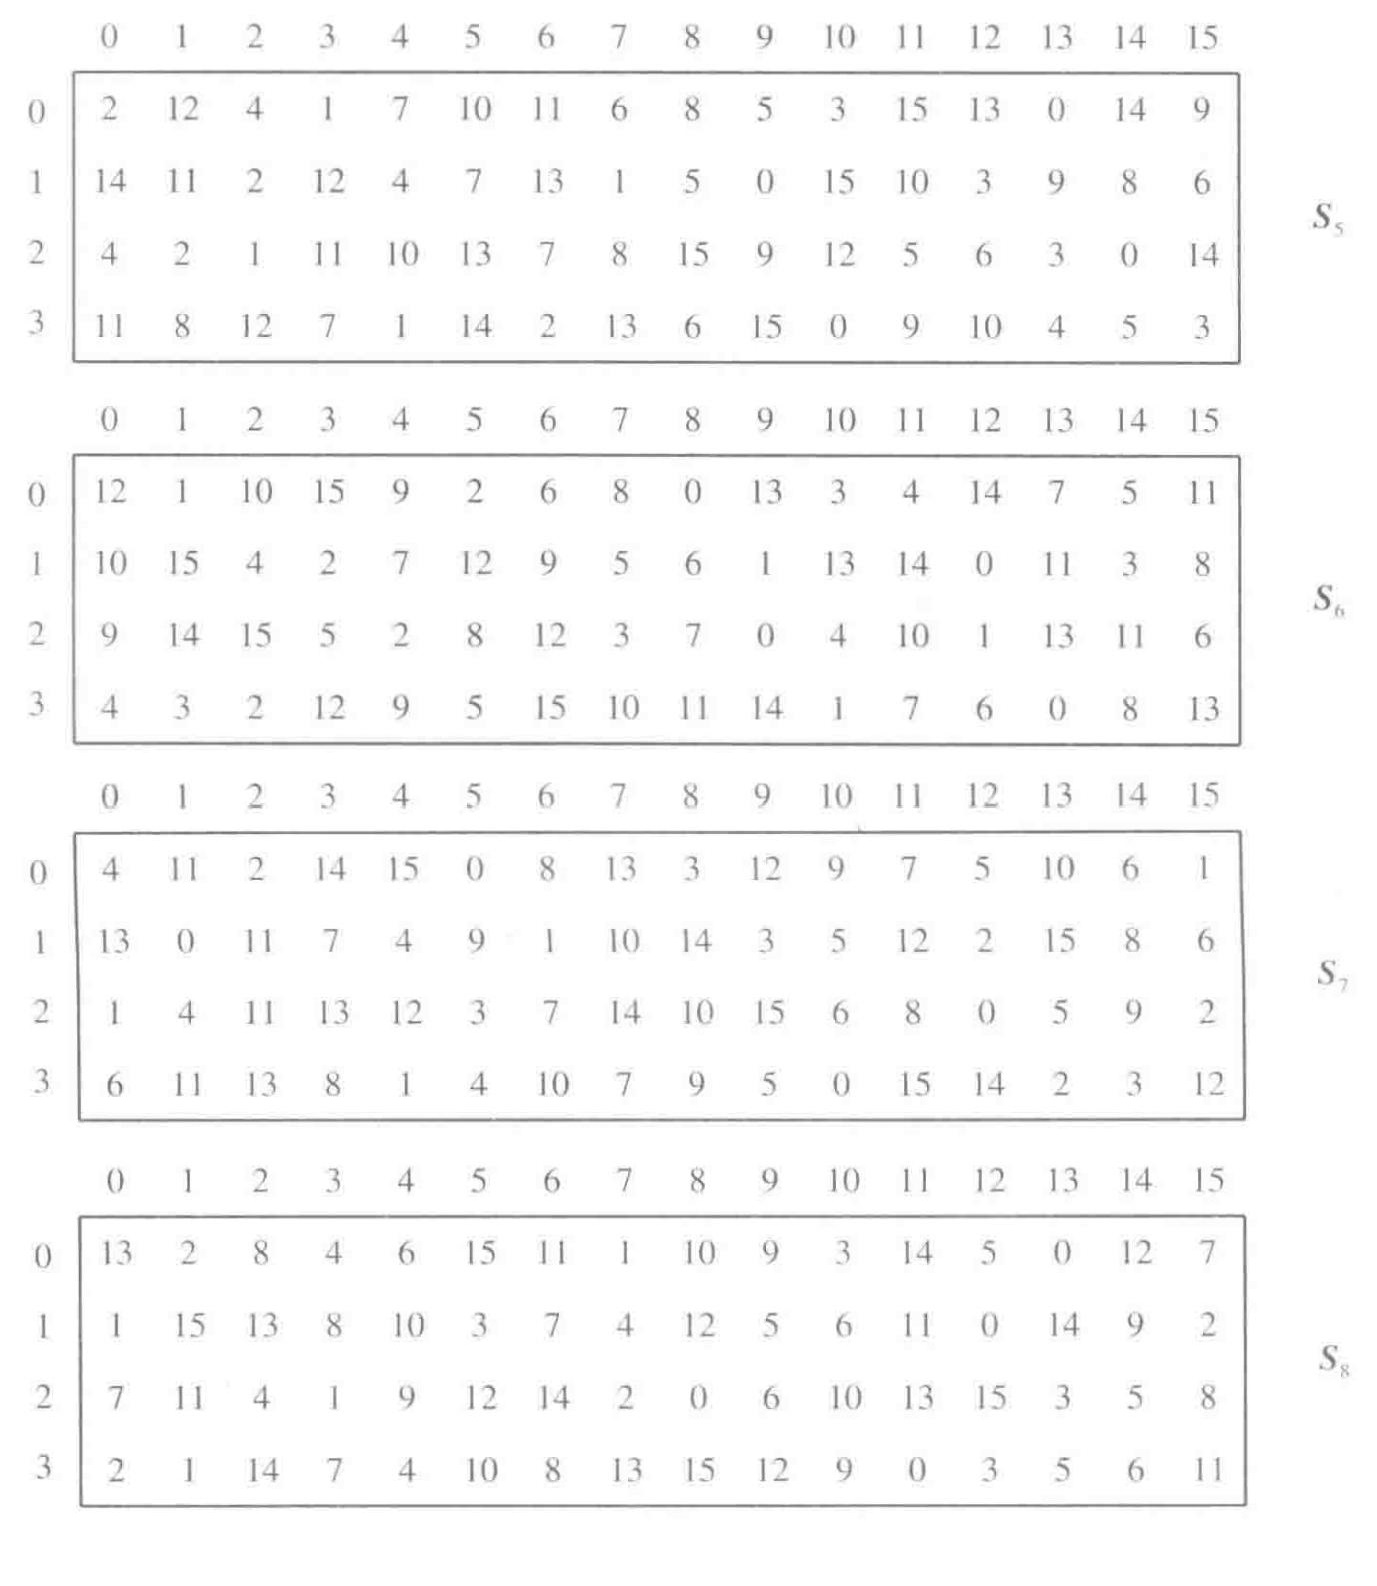
\includegraphics[width=\textwidth]{S_2.jpg}
                    \label{fig:subfig2}
                \end{subfigure}
                \caption{S盒代替矩阵}
                \label{fig:subfigures}
            \end{figure}
            进行S盒运算的整体代替代码如下所示
            \lstinputlisting[caption={S盒整体代码},captionpos=b,firstline=60, lastline=67]{E:/Python_code/codes/密码学/lab_1/F.py}
            单个S盒的运算代码如下所示
            \lstinputlisting[caption={单个S盒整体代码},captionpos=b,firstline=16, lastline=57]{E:/Python_code/codes/密码学/lab_1/F.py}
\newpage
        \subsubsection{置换运算P}
            置换运算P将S盒输出的32位数据进行打乱重排,得到32位的加密函数输出,从而达到将S盒的混淆作用扩散的目的。\par
            进行置换运算P的代码如下所示
            \lstinputlisting[caption={置换运算P},captionpos=b,firstline=30, lastline=36]{E:/Python_code/codes/密码学/lab_1/place_change.py}
\newpage
    \subsection{DES加密过程完整实现}
        DES的整个加密过程用流程图表示如下图所示
        \begin{figure}[H]
            \centering
            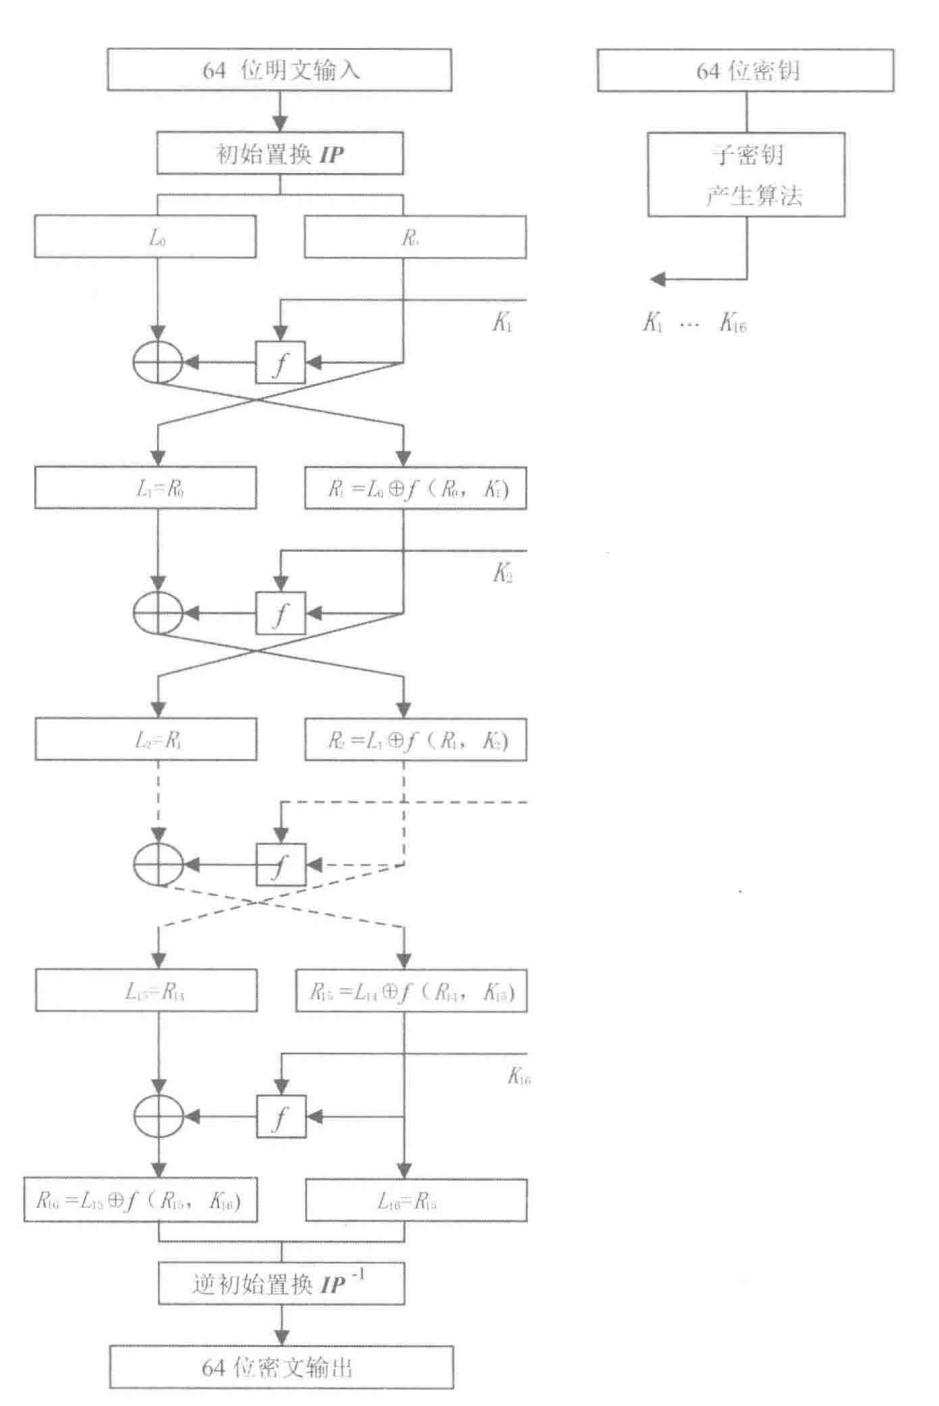
\includegraphics[width=9cm]{DES_1.jpg}
            \bottomcaption{\xiaowuhao{DES整体流程图}}
        \end{figure}
        整个DES加密过程用数学公式表示\par
        $\begin{cases}
            L_{i}=R_{i-1}\\ R_{i}=L_{i-1}\oplus f\left( R_{i-1},k_{i}\right) \\ i=1,2,3,\ldots ,16
        \end{cases}$
        \subsubsection{子密钥产生算法}
            64位密钥经子密钥产生算法产生出16个子密钥:$K_{1},K_{2},\ldots,K_{16}$,分别供第一次,第二次,...,第十六次加密迭代使用。
        \subsubsection{初始置乱IP}
            64位明文首先经过初始置换IP(Initial permutation),将数据打乱重新排列并分成左右两半。左边32位构成$L_{0}$,左边32位构成$R_{0}$
        \subsubsection{初次迭代}
            由加密函数f实现子密钥$K_{1}$ 对$R_{0}$的加密,结果为32位的数据组$f(R_{0},K_{1})$,再与$L_{0}$进行异或运算,又得到一个32位的数据组$L_{0}\oplus f(R_{0},K_{1})$。
            以$L_{0}\oplus f(R_{0},K_{1})$作为第二次加密迭代的$R_{1}$,以$R_{0}$作为第二次加密迭代的$L_{1}$。至此,第一次加密迭代结束。
        \subsubsection{16次加密迭代}
            第二次加密迭代至第十六次加密迭代分别用子密钥$K_{2},\ldots,K_{16}$进行,其过程与第一次加密迭代相同。
        \subsubsection{逆初始置换$IP^{-1} $}
            第十六次加密迭代结束后,产生一个64位的数据组。以$R_{16}$作为其左边32位,以$L_{16}$作为其右边32位,两者合并再经过逆初始置换$IP^{-1} $,将数据重新排列,便得到64位密文。至此加密过程全部结束。\par
\newpage
        整个DES加密函数的代码如下所示
        \lstinputlisting[caption={DES加密主函数},captionpos=b,firstline=16, lastline=33]{E:/Python_code/codes/密码学/lab_1/DES.py}
\newpage
    \subsection{DES解密过程实现}
        由于DES的运算是对和运算,所以解密和加密可共用同一个运算,只是子密钥使用的顺序不同。
        把64位密文当作明文输入,而且第一次解密迭代使用子密钥$K_{16}$,第二次解密迭代使用子密钥$K_{15}$,第十六次解密迭代使用子密钥$K_{1}$,最后的输出便是64位明文。
        解密过程可用如下的数学公式描述:\par
        $\begin{cases}
            R_{i-1}=L_{i}\\ L_{i-1}=R_{i}\oplus f\left( R_{i-1},k_{i}\right) \\ i=16,15,14,\ldots ,1
        \end{cases}$\par
        解密过程的代码如下所示
        \lstinputlisting[caption={DES解密主函数},captionpos=b,firstline=36, lastline=61]{E:/Python_code/codes/密码学/lab_1/DES.py}

    \subsection{DES的S盒密码学特性}
        通过编程实现或者手工计算,试验证S盒的以下准则:定义S盒的输入为X,输出为Y(X和Y都以二进制表示)
        \subsubsection{输出不是输入的线性和仿射函数}
            (1)首先证明线性函数,令$x_{1}=110001,x_{2}=110010,X3=110011$,使用S盒1,分别求得其输出值如下图所示
            \begin{figure}[H]
                \centering
                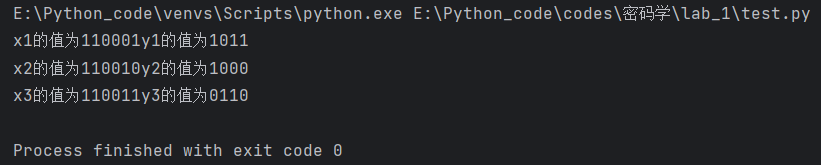
\includegraphics[width=9cm]{test_result_1.png}
                \bottomcaption{\xiaowuhao{验证线性函数运行结果}}
            \end{figure}
            得出的$y_{1}=1011,y_{2}=1000,y_{3}=0110$,x的值每位加1递增,得到的y的值却并不存在线性关系,由此可以证明S盒的输出不是线性函数\par

            (1)接下来证明仿射函数,令$x_{1}=0b110010=0d2,x_{2}=0b110100=0d4,z1=\alpha x_{1}+\beta x_{2},z2=\alpha x_{1},z3=\beta x_{2},\alpha =0.5,\beta =0.5$,
            求得$y_{1}=f(z1),y_{2}=f(z2),y_{3}=f(z3)$的结果如下图所示
            \begin{figure}[H]
                \centering
                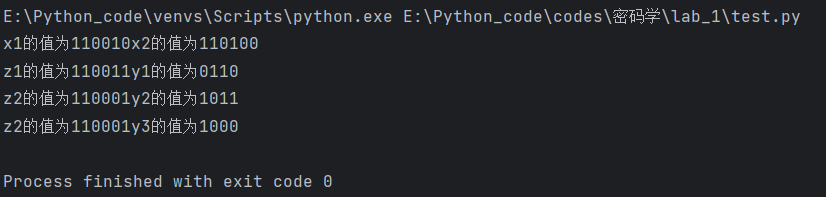
\includegraphics[width=9cm]{test_result_1_2.png}
                \bottomcaption{\xiaowuhao{验证仿射函数运行结果}}
            \end{figure}
            根据计算出的结果$y_{1}=0b0110,y_{2}=0b1011,y_{3}=0b1000$,可以得出结论$y_{1}\ne y_{2}+y_{3}$,与仿射函数的定义向矛盾,所以S盒不是仿射函数。

        \subsubsection{任意改变输入中的一位,输出至少有两位发生变化}
            令$x_{1}=110010,x_{2}=100010$,使用S盒2,分别求得其输出值$y_{1},y_{2}$并对$y_{1},y_{2}$进行异或运算,得到的结果如下图所示
            \begin{figure}[H]
                \centering
                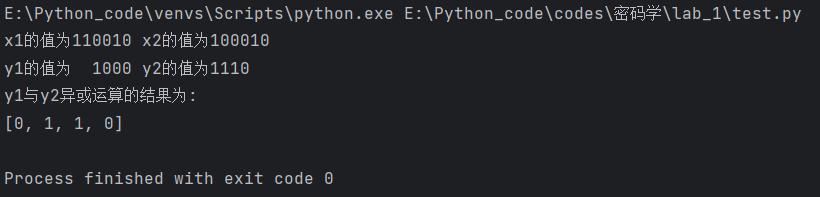
\includegraphics[width=9cm]{test_result_2.png}
                \bottomcaption{\xiaowuhao{验正修改一位输入后的输出变化的运行结果}}
            \end{figure}
            通过观察结果发现,异或运算的结果为0110,输出有两位发生变化,得证。

        \subsubsection{对于任何S盒和任何输入x,$S(x)$和$S(x\oplus 001100)$至少有两位不同,这里x是一个6位的二进制串}
            令$x_{1}=110010,x_{2}=x_{1}\oplus 001100=111110$分别求得其输出值$y_{1},y_{2}$并对$y_{1},y_{2}$进行异或运算,得到的结果如下图所示
            \begin{figure}[H]
                \centering
                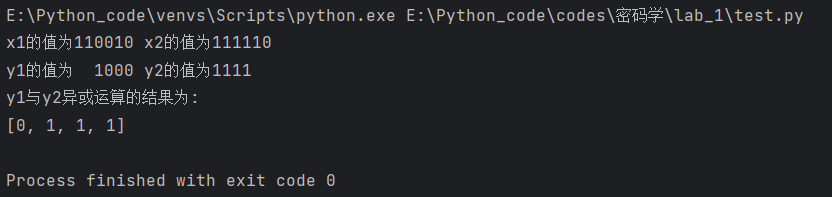
\includegraphics[width=9cm]{test_result_3.png}
                \bottomcaption{\xiaowuhao{$x\oplus 001100$后的输出变化的运行结果}}
            \end{figure}
            通过观察结果发现,异或运算的结果为0111,输出有3位发生变化,得证。

        \subsubsection{对于任何S盒和任何输入x,以及$y,z\in GF(2),S(x)\ne S(x\oplus 11yz00)$,这里x是一个6位的二进制串}
            令$x_{1}=110010,x_{2}=x_{1}\oplus 110000,x_{3}=x_{1}\oplus 110100,x_{4}=x_{1}\oplus 111000,x_{5}=x_{1}\oplus 111100$
            分别求得其输出值$y_{1},y_{2},y_{3},y_{4},y_{5}$并对$y_{1}$与其余四个输出结果进行异或运算,得到的结果如下图所示

            \begin{figure}[H]
                \centering
                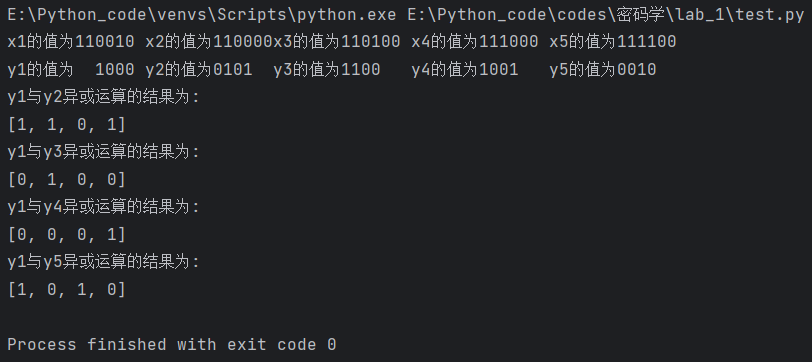
\includegraphics[width=9cm]{test_result_4.png}
                \bottomcaption{\xiaowuhao{$x\oplus 11yz00$后的输出变化的运行结果}}
            \end{figure}
            通过观察结果发现,$y_{1}$与其余四个输出结果进行异或运算的结果分别为1101,0100,0001,1010,均不为全0,得证。

        \subsubsection{保持输入中的1位不变,其余5位变化,输出中的0和1的个数接近相等。}
            令$x_{1}=110010,x_{2}=101101$分别求得其输出值$y_{1},y_{2}$并统计0和1的个数得到的结果如下图所示
            \begin{figure}[H]
                \centering
                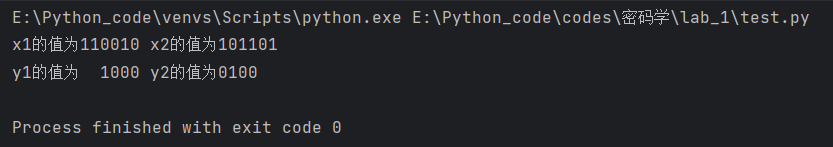
\includegraphics[width=9cm]{test_result_5.png}
                \bottomcaption{\xiaowuhao{改变输入中的5位后的输出变化的运行结果}}
            \end{figure}
            通过观察结果发现,y1的值为1000,y2的值为0100,两个输出的0和1的个数相同,得证。
        \subsubsection{根据上面得出的结果试说明S盒对于DES的安全性影响。}
            (1)非线性变换:S盒是DES中的一个非线性变换,它将输入的6位数据映射到4位输出。这种非线性性质增加了密码算法的复杂性,
            使得密码分析变得更加困难。如果S盒是线性的,那么DES的安全性将大大降低,因为线性变换容易受到线性密码分析的攻击。\par
            (2)混淆和扩散:S盒的设计旨在实现数据的混淆和扩散。这意味着输入中的每一位都对输出产生影响,
            同时输出的每一位都依赖于输入的多个位。这有助于确保在每一轮DES加密中都发生了广泛的变化,增加了密码的复杂性和安全性。\par
            (3)防止经典攻击:S盒设计的目标之一是抵御一些经典的密码分析攻击,例如差分密码分析和线性密码分析。
            合理设计的S盒可以使这些攻击变得非常困难,要求攻击者大量的计算和数据。\par
            (4)增加密钥空间:DES中有8个不同的S盒,每个S盒都有自己的置换表。这些S盒的组合扩展了DES的密钥空间,使得暴力攻击变得更加困难,因为攻击者需要尝试大量的密钥组合。\par

    \subsection{验证教材P64页实例}
        因为在教材中的密钥并未涉及到将第8位做奇偶校验,所以在验证的过程中直接将给出的密钥作为已经处理好的密钥二进制数据进行验证。
        \subsubsection{密钥拓展}
            将给出的密钥输入程序后进行调试,置换选择1的结果保存在变量key1中,key1的值如下图所示,与教材中给出的置换选择1的值相同。\par
            \begin{figure}[H]
                \centering
                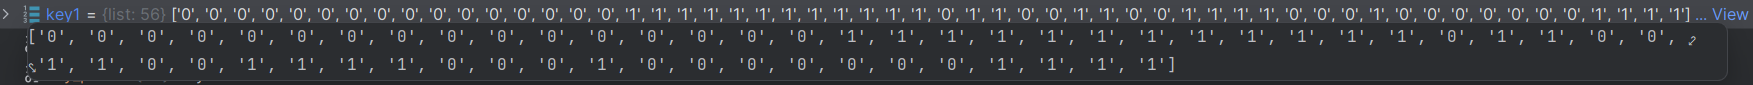
\includegraphics[width=15cm]{置换选择1.png}
                \bottomcaption{\xiaowuhao{置换选择1的结果}}
            \end{figure}
\newpage
            计算出的C0和D0的值保存到二维列表key\_c和key\_d的中如下图所示,与教材中给出的值相同
            \begin{figure}[H]
                \centering
                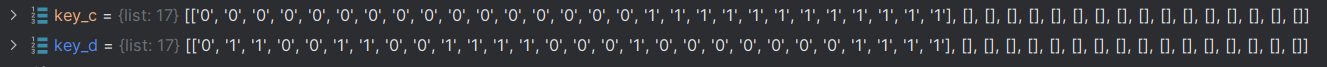
\includegraphics[width=15cm]{C0D0.png}
                \bottomcaption{\xiaowuhao{计算得到的C0和D0的结果}}
            \end{figure}
            继续调试程序得到所有的C的值如下图所示,与教材中给出的所有C的值相同
            \begin{figure}[H]
                \centering
                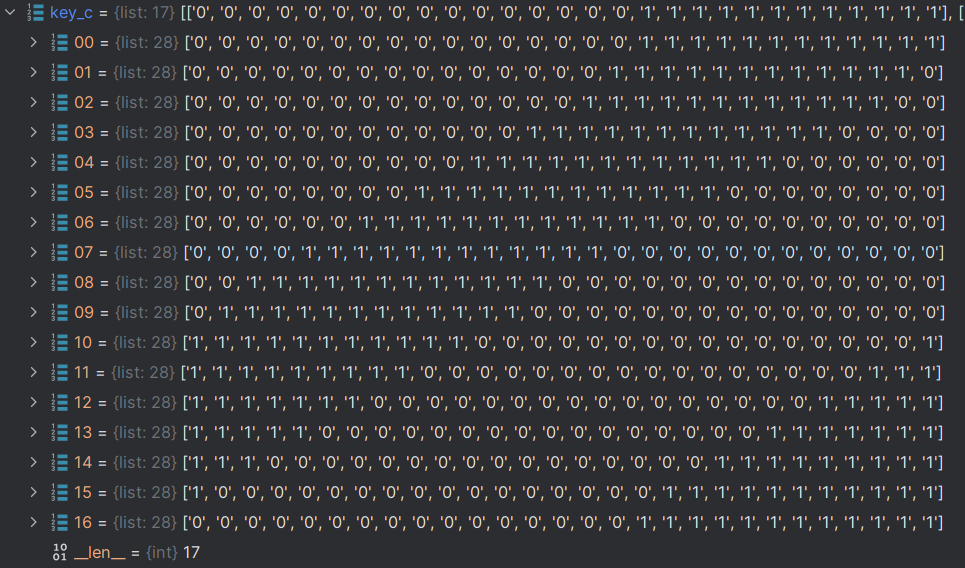
\includegraphics[width=9cm]{key_c.png}
                \bottomcaption{\xiaowuhao{调试程序得到所有的C的值}}
            \end{figure}
            继续调试程序得到的所有的D的值如下图所示,与教材中给出的所有的D的值相同
            \begin{figure}[H]
                \centering
                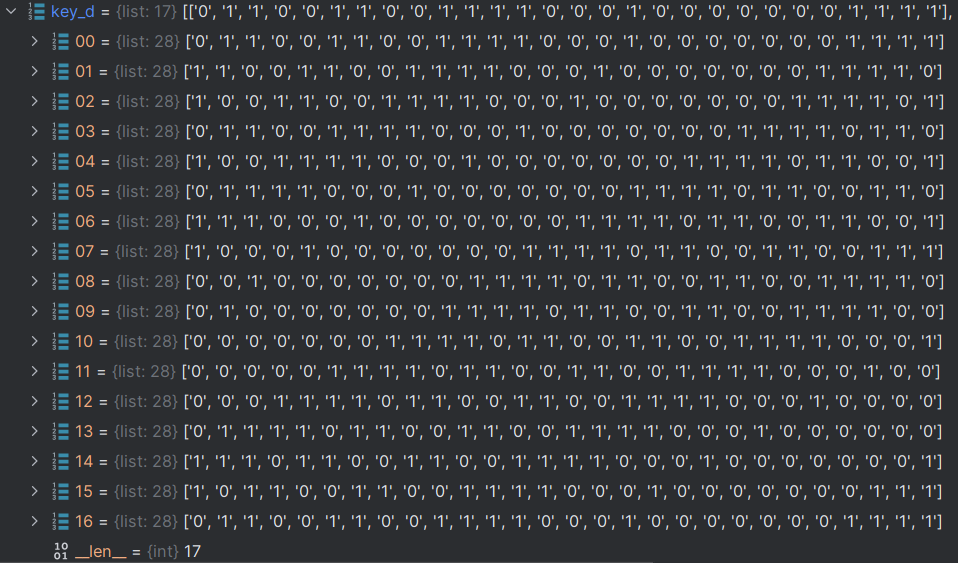
\includegraphics[width=9cm]{key_d.png}
                \bottomcaption{\xiaowuhao{调试程序得到所有的D的值}}
            \end{figure}
\newpage
            继续调试程序得到的所有的子密钥的值如下图所示,与教材中给出的所有的子密钥的值相同
            \begin{figure}[H]
                \centering
                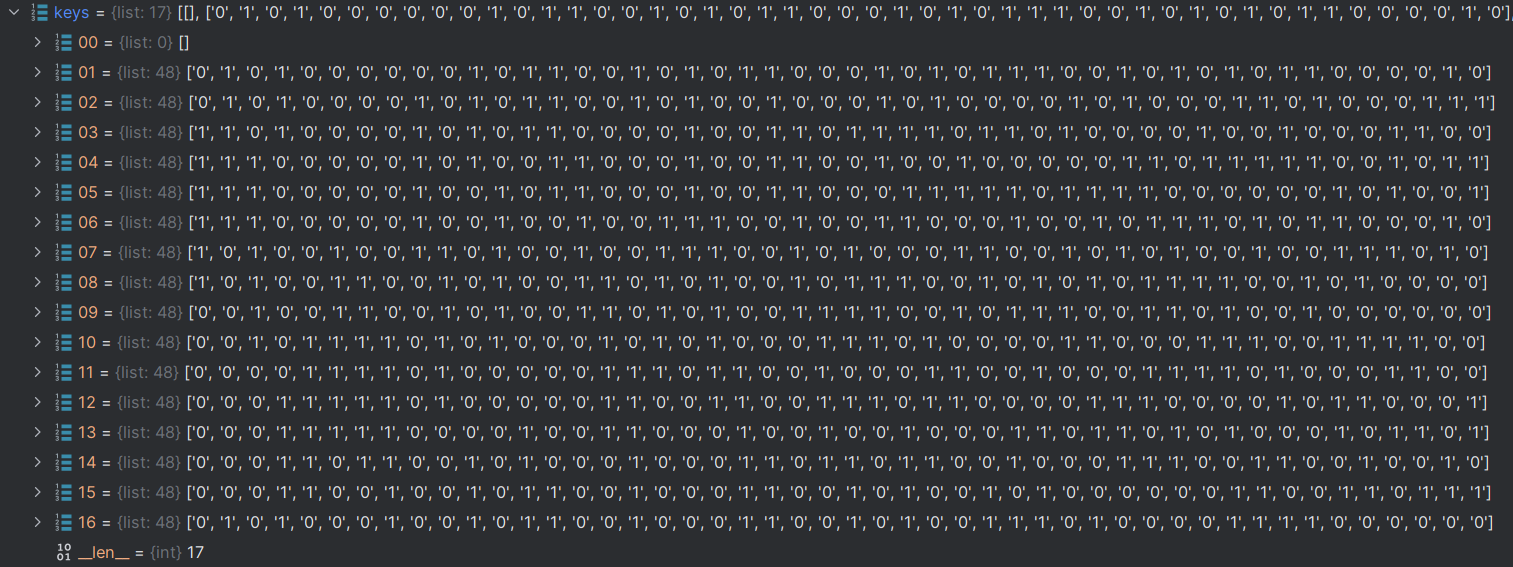
\includegraphics[width=11cm]{keys.png}
                \bottomcaption{\xiaowuhao{调试程序得到所有的子密钥的值}}
            \end{figure}
        \subsubsection{加密过程}
            教材中给出的明文序列为01234567,在程序中使用该序列作为明文,继续使用密钥拓展过程的密钥作为本次实验的密钥。\par
            调试程序得到初始置换后的结果如下图所示,与教材中给出的值相同
            \begin{figure}[H]
                \centering
                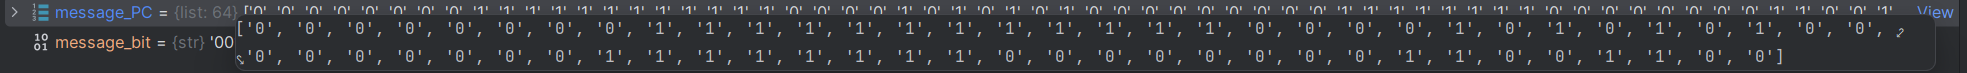
\includegraphics[width=15cm]{初始置换.png}
                \bottomcaption{\xiaowuhao{初始置换后结果}}
            \end{figure}
            调试程序得到L0和R0的结果如下图所示,与教材中给出的相同
            \begin{figure}[H]
                \centering
                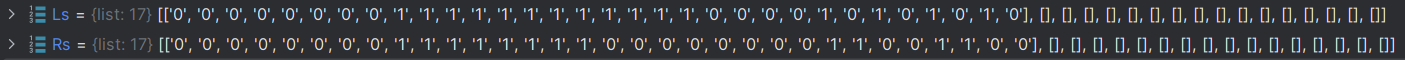
\includegraphics[width=15cm]{L0R0.png}
                \bottomcaption{\xiaowuhao{得到L0和R0的结果}}
            \end{figure}
\newpage
            第1轮循环得到的结果如下图所示,其中,F函数的32位输入保存在变量R中,选择运算的结果保存在变量E中,子密钥k1保存在变量k中,
            子密钥加后的结果保存在变量S\_input中,S盒输出的结果保存在变量S\_output中,P置乱后的结果保存在返回值result中,与教材中给出的值相同
            \begin{figure}[H]
                \centering
                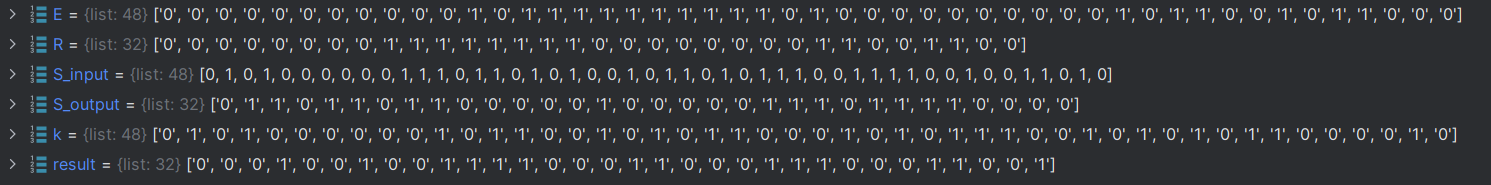
\includegraphics[width=15cm]{N1.png}
                \bottomcaption{\xiaowuhao{第1轮循环的结果}}
            \end{figure}
            第2轮循环后得到的结果如下图所示,与教材中给出的值相同
            \begin{figure}[H]
                \centering
                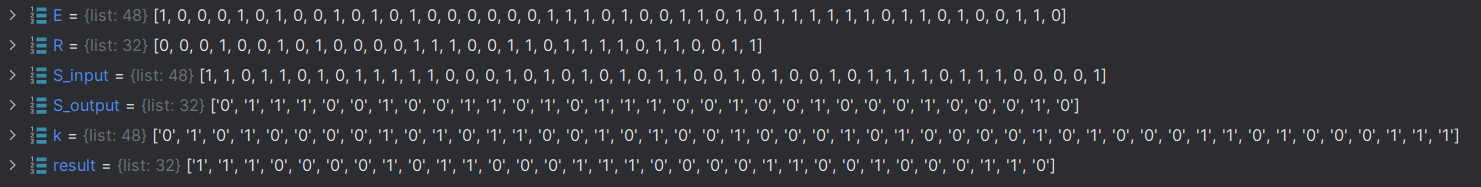
\includegraphics[width=15cm]{N2.png}
                \bottomcaption{\xiaowuhao{第2轮循环的结果}}
            \end{figure}
            第3轮循环后得到的结果如下图所示,与教材中给出的值相同
            \begin{figure}[H]
                \centering
                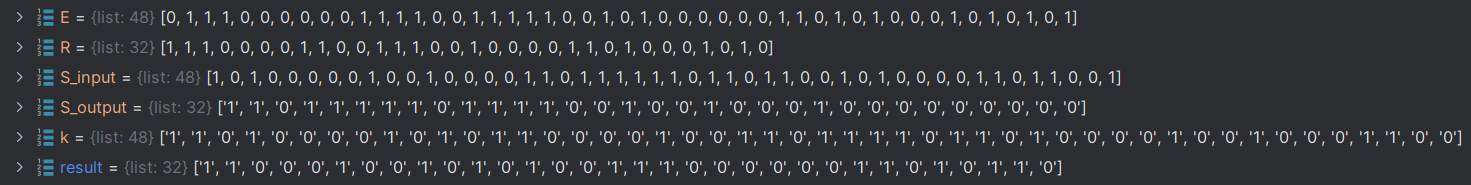
\includegraphics[width=15cm]{N3.png}
                \bottomcaption{\xiaowuhao{第3轮循环的结果}}
            \end{figure}
            第4轮循环后得到的结果如下图所示,与教材中给出的值相同
            \begin{figure}[H]
                \centering
                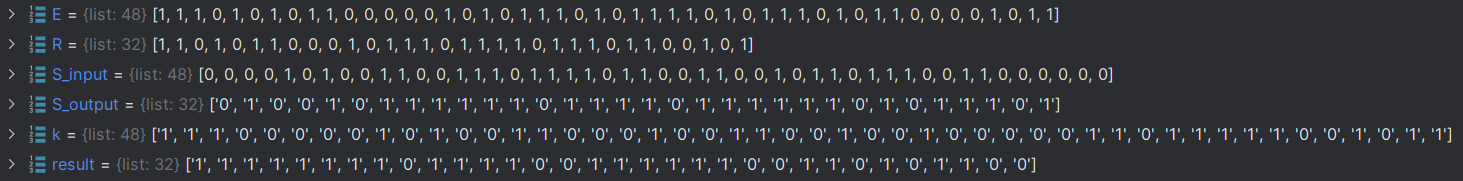
\includegraphics[width=15cm]{N4.png}
                \bottomcaption{\xiaowuhao{第4轮循环的结果}}
            \end{figure}
\newpage
            第5轮循环后得到的结果如下图所示,与教材中给出的值相同
            \begin{figure}[H]
                \centering
                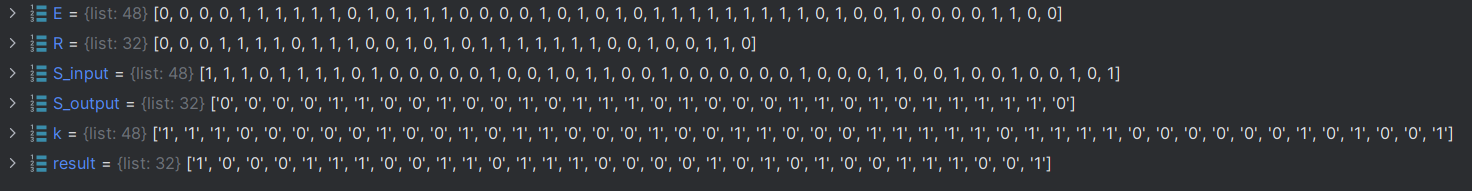
\includegraphics[width=15cm]{N5.png}
                \bottomcaption{\xiaowuhao{第5轮循环的结果}}
            \end{figure}
            第6轮循环后得到的结果如下图所示,与教材中给出的值相同
            \begin{figure}[H]
                \centering
                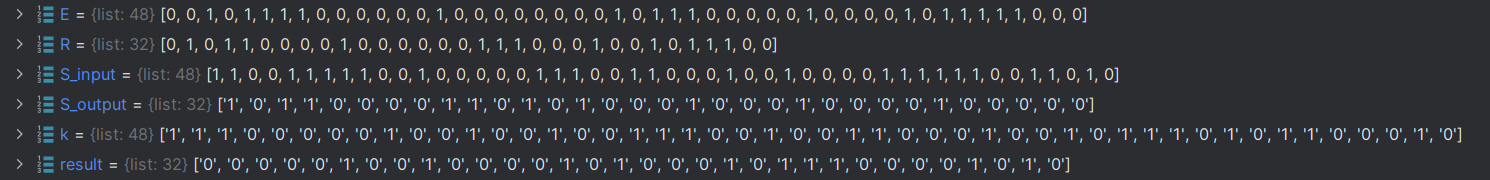
\includegraphics[width=15cm]{N6.png}
                \bottomcaption{\xiaowuhao{第6轮循环的结果}}
            \end{figure}
            第7轮循环后得到的结果如下图所示,与教材中给出的值相同
            \begin{figure}[H]
                \centering
                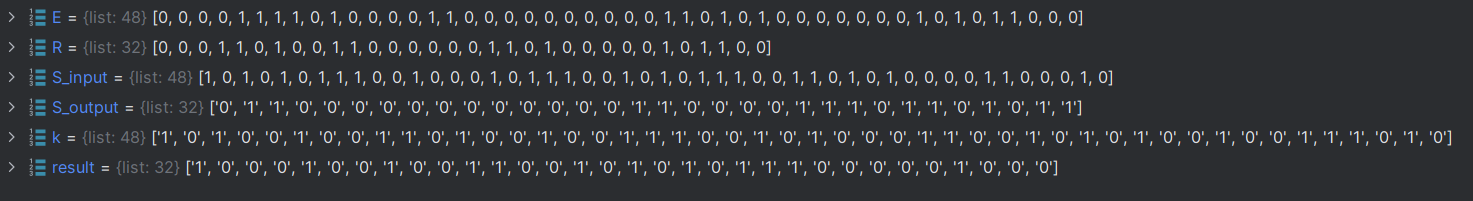
\includegraphics[width=15cm]{N7.png}
                \bottomcaption{\xiaowuhao{第7轮循环的结果}}
            \end{figure}
            第8轮循环后得到的结果如下图所示,与教材中给出的值相同
            \begin{figure}[H]
                \centering
                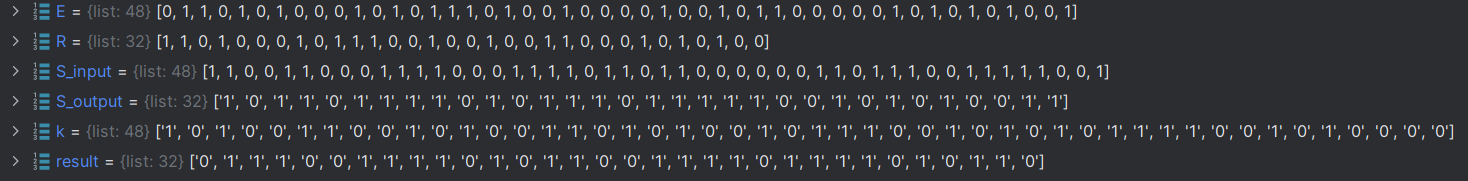
\includegraphics[width=15cm]{N8.png}
                \bottomcaption{\xiaowuhao{第8轮循环的结果}}
            \end{figure}
            第9轮循环后得到的结果如下图所示,与教材中给出的值相同
            \begin{figure}[H]
                \centering
                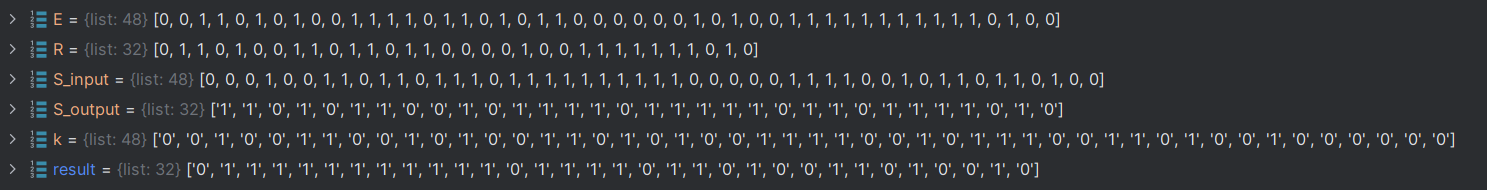
\includegraphics[width=15cm]{N9.png}
                \bottomcaption{\xiaowuhao{第9轮循环的结果}}
            \end{figure}
            第10轮循环后得到的结果如下图所示,与教材中给出的值相同
            \begin{figure}[H]
                \centering
                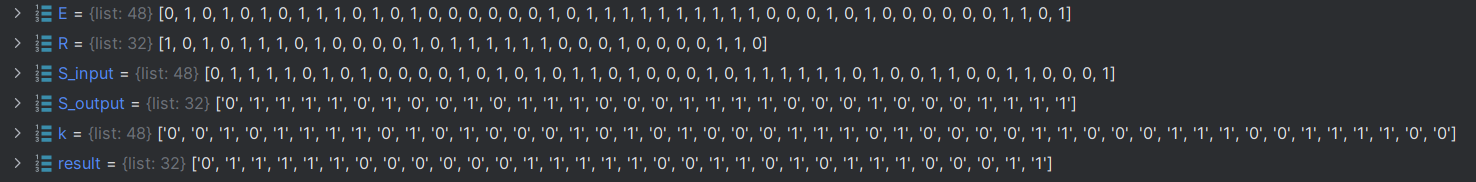
\includegraphics[width=15cm]{N10.png}
                \bottomcaption{\xiaowuhao{第10轮循环的结果}}
            \end{figure}
            第11轮循环后得到的结果如下图所示,与教材中给出的值相同
            \begin{figure}[H]
                \centering
                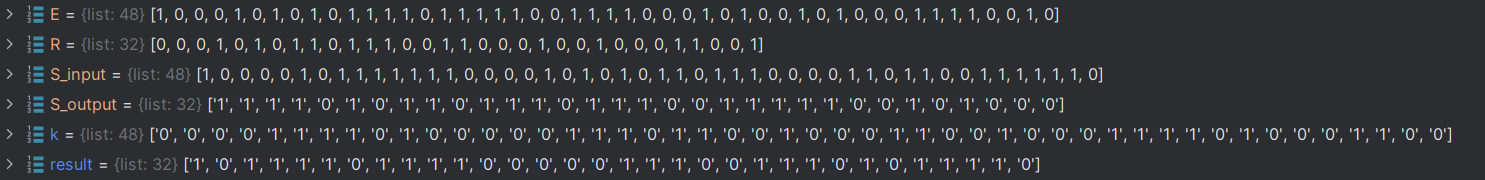
\includegraphics[width=15cm]{N11.png}
                \bottomcaption{\xiaowuhao{第11轮循环的结果}}
            \end{figure}
            第12轮循环后得到的结果如下图所示,与教材中给出的值相同
            \begin{figure}[H]
                \centering
                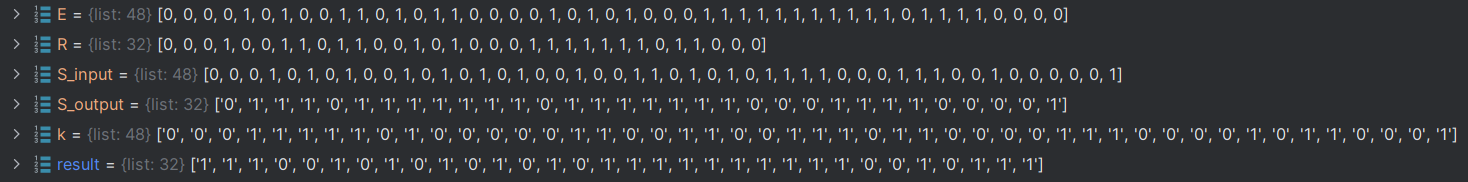
\includegraphics[width=15cm]{N12.png}
                \bottomcaption{\xiaowuhao{第12轮循环的结果}}
            \end{figure}
            第13轮循环后得到的结果如下图所示,与教材中给出的值相同
            \begin{figure}[H]
                \centering
                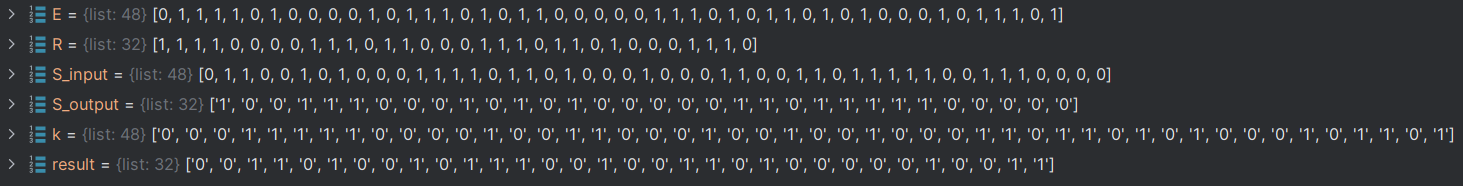
\includegraphics[width=15cm]{N13.png}
                \bottomcaption{\xiaowuhao{第13轮循环的结果}}
            \end{figure}
            第14轮循环后得到的结果如下图所示,与教材中给出的值相同
            \begin{figure}[H]
                \centering
                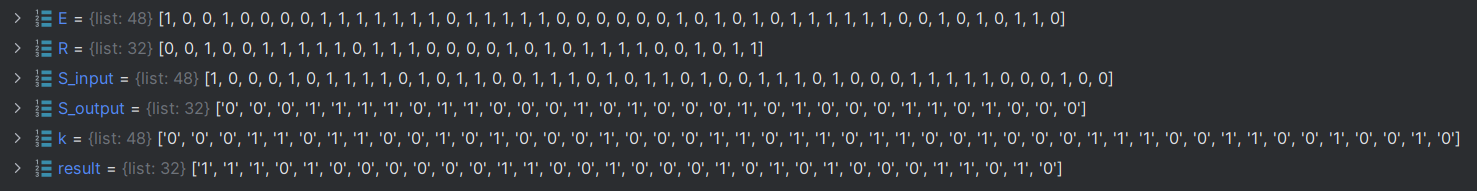
\includegraphics[width=15cm]{N14.png}
                \bottomcaption{\xiaowuhao{第14轮循环的结果}}
            \end{figure}
\newpage
            第15轮循环后得到的结果如下图所示,与教材中给出的值相同
            \begin{figure}[H]
                \centering
                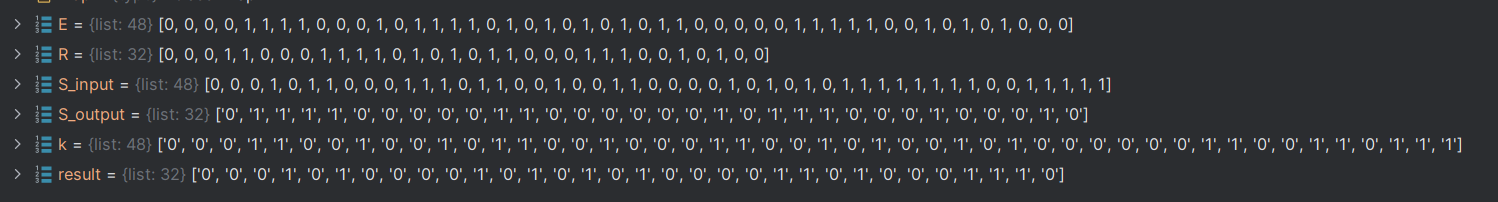
\includegraphics[width=15cm]{N15.png}
                \bottomcaption{\xiaowuhao{第15轮循环的结果}}
            \end{figure}
            第16轮循环后得到的结果如下图所示,与教材中给出的值相同
            \begin{figure}[H]
                \centering
                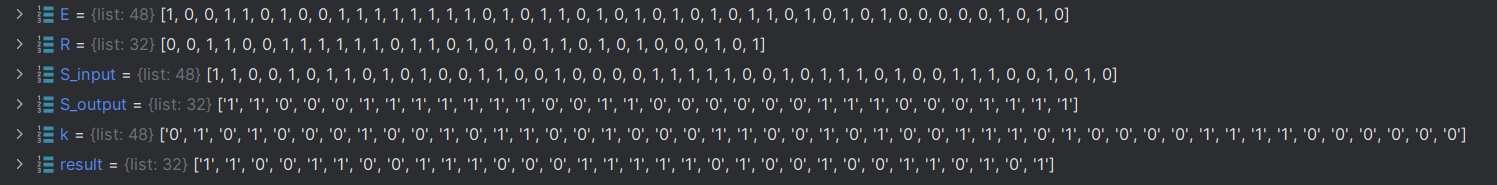
\includegraphics[width=15cm]{N16.png}
                \bottomcaption{\xiaowuhao{第16轮循环的结果}}
            \end{figure}
            继续调试程序得到所有的L的结果如下图所示,与教材中给出的值一致
            \begin{figure}[H]
                \centering
                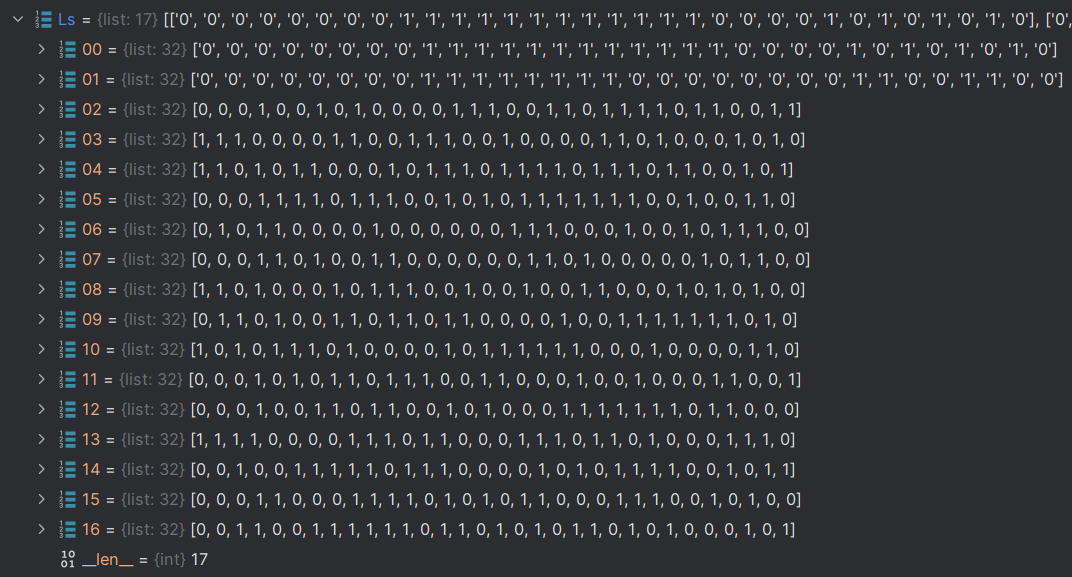
\includegraphics[width=9cm]{L.png}
                \bottomcaption{\xiaowuhao{L的值}}
            \end{figure}
            继续调试程序得到所有的R的结果如下图所示,与教材中给出的值一致
            \begin{figure}[H]
                \centering
                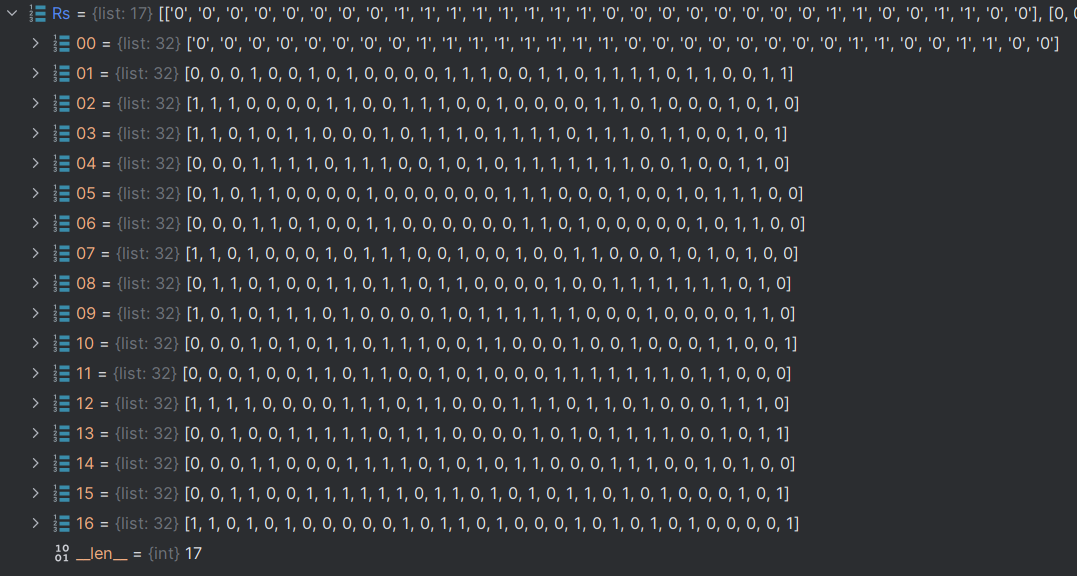
\includegraphics[width=9cm]{R.png}
                \bottomcaption{\xiaowuhao{R的值}}
            \end{figure}
            继续调试函数得到逆初始置换的结果即密文如下图所示
            \begin{figure}[H]
                \centering
                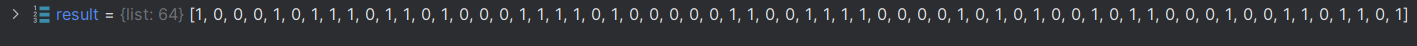
\includegraphics[width=15cm]{密文.png}
                \bottomcaption{\xiaowuhao{64位密文}}
            \end{figure}
        \subsubsection{解密过程}
            教材中给出的密文序列是机密过程产生的密文,在程序中使用该序列作为密文,继续使用密钥拓展过程的密钥作为本次实验的密钥。\par
            调试程序得到初始置换后的结果如下图所示,与教材中给出的值相同
            \begin{figure}[H]
                \centering
                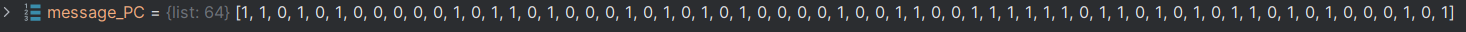
\includegraphics[width=15cm]{d初始置换.png}
                \bottomcaption{\xiaowuhao{初始置换后结果}}
            \end{figure}
            调试程序得到L0和R0的结果如下图所示,与教材中给出的相同
            \begin{figure}[H]
                \centering
                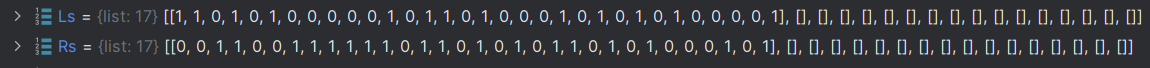
\includegraphics[width=15cm]{dL0R0.png}
                \bottomcaption{\xiaowuhao{得到L0和R0的结果}}
            \end{figure}
            第1轮循环得到的结果如下图所示,其中,F函数的32位输入保存在变量R中,选择运算的结果保存在变量E中,子密钥k1保存在变量k中,
            子密钥加后的结果保存在变量S\_input中,S盒输出的结果保存在变量S\_output中,P置乱后的结果保存在返回值result中,与教材中给出的值相同
            \begin{figure}[H]
                \centering
                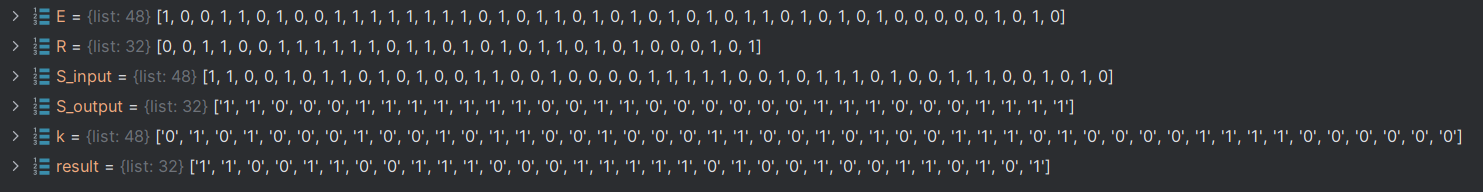
\includegraphics[width=15cm]{dN1.png}
                \bottomcaption{\xiaowuhao{第1轮循环的结果}}
            \end{figure}
\newpage
            第2轮循环后得到的结果如下图所示,与教材中给出的值相同
            \begin{figure}[H]
                \centering
                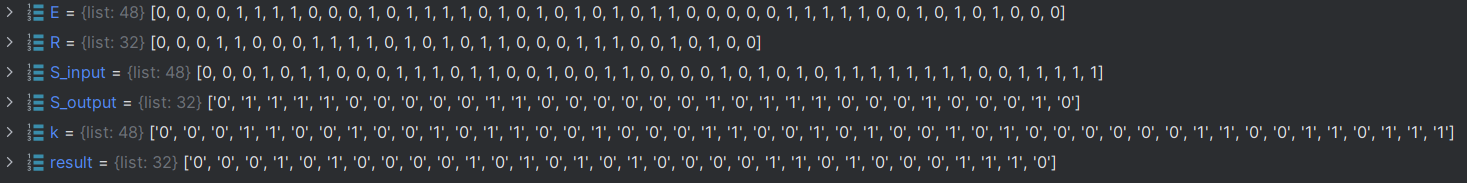
\includegraphics[width=15cm]{dN2.png}
                \bottomcaption{\xiaowuhao{第2轮循环的结果}}
            \end{figure}
            第3轮循环后得到的结果如下图所示,与教材中给出的值相同
            \begin{figure}[H]
                \centering
                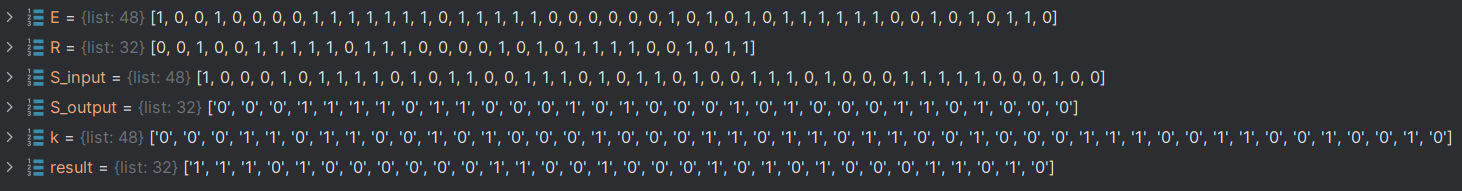
\includegraphics[width=15cm]{dN3.png}
                \bottomcaption{\xiaowuhao{第3轮循环的结果}}
            \end{figure}
            第4轮循环后得到的结果如下图所示,与教材中给出的值相同
            \begin{figure}[H]
                \centering
                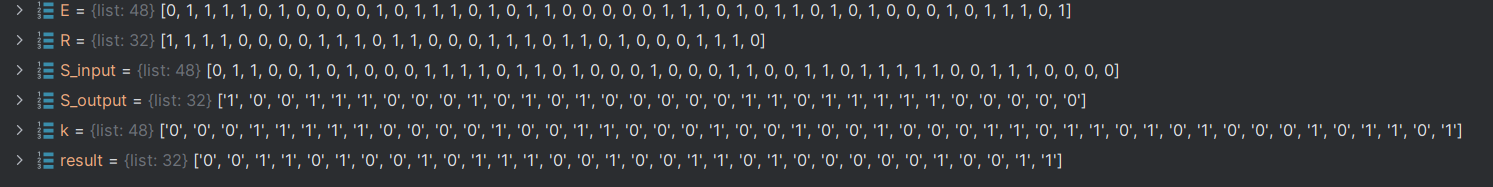
\includegraphics[width=15cm]{dN4.png}
                \bottomcaption{\xiaowuhao{第4轮循环的结果}}
            \end{figure}
            第5轮循环后得到的结果如下图所示,与教材中给出的值相同
            \begin{figure}[H]
                \centering
                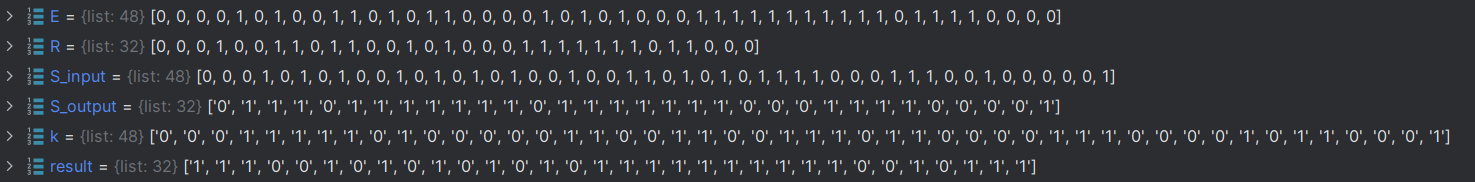
\includegraphics[width=15cm]{dN5.png}
                \bottomcaption{\xiaowuhao{第5轮循环的结果}}
            \end{figure}
            第6轮循环后得到的结果如下图所示,与教材中给出的值相同
            \begin{figure}[H]
                \centering
                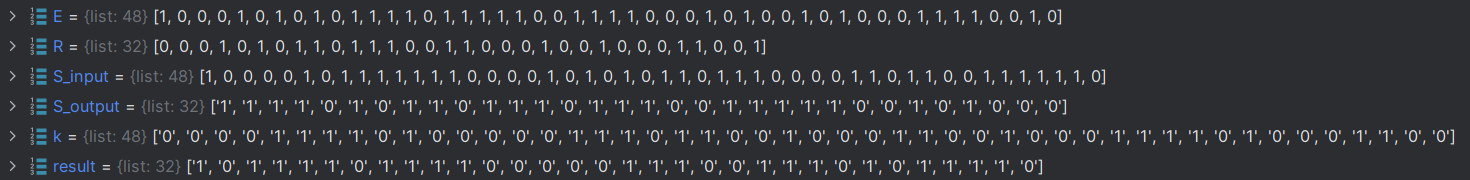
\includegraphics[width=15cm]{dN6.png}
                \bottomcaption{\xiaowuhao{第6轮循环的结果}}
            \end{figure}
\newpage
            第7轮循环后得到的结果如下图所示,与教材中给出的值相同
            \begin{figure}[H]
                \centering
                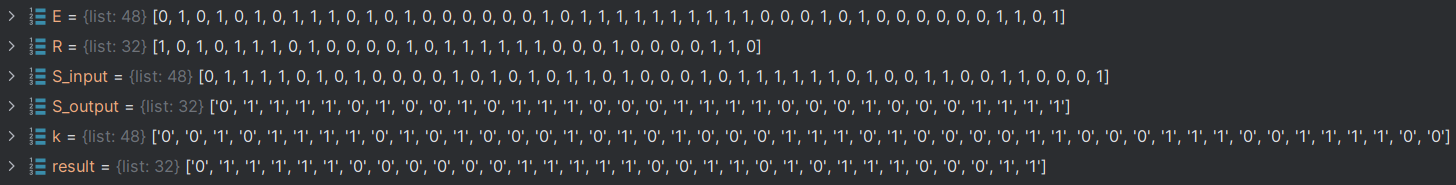
\includegraphics[width=15cm]{dN7.png}
                \bottomcaption{\xiaowuhao{第7轮循环的结果}}
            \end{figure}
            第8轮循环后得到的结果如下图所示,与教材中给出的值相同
            \begin{figure}[H]
                \centering
                \includegraphics[width=15cm]{dN8.png}
                \bottomcaption{\xiaowuhao{第8轮循环的结果}}
            \end{figure}
            第9轮循环后得到的结果如下图所示,与教材中给出的值相同
            \begin{figure}[H]
                \centering
                \includegraphics[width=15cm]{dN9.png}
                \bottomcaption{\xiaowuhao{第9轮循环的结果}}
            \end{figure}
            第10轮循环后得到的结果如下图所示,与教材中给出的值相同
            \begin{figure}[H]
                \centering
                \includegraphics[width=15cm]{dN10.png}
                \bottomcaption{\xiaowuhao{第10轮循环的结果}}
            \end{figure}
            第11轮循环后得到的结果如下图所示,与教材中给出的值相同
            \begin{figure}[H]
                \centering
                \includegraphics[width=15cm]{dN11.png}
                \bottomcaption{\xiaowuhao{第11轮循环的结果}}
            \end{figure}
\newpage
            第12轮循环后得到的结果如下图所示,与教材中给出的值相同
            \begin{figure}[H]
                \centering
                \includegraphics[width=15cm]{dN12.png}
                \bottomcaption{\xiaowuhao{第12轮循环的结果}}
            \end{figure}
            第13轮循环后得到的结果如下图所示,与教材中给出的值相同
            \begin{figure}[H]
                \centering
                \includegraphics[width=15cm]{dN13.png}
                \bottomcaption{\xiaowuhao{第13轮循环的结果}}
            \end{figure}
            第14轮循环后得到的结果如下图所示,与教材中给出的值相同
            \begin{figure}[H]
                \centering
                \includegraphics[width=15cm]{dN14.png}
                \bottomcaption{\xiaowuhao{第14轮循环的结果}}
            \end{figure}
            第15轮循环后得到的结果如下图所示,与教材中给出的值相同
            \begin{figure}[H]
                \centering
                \includegraphics[width=15cm]{dN15.png}
                \bottomcaption{\xiaowuhao{第15轮循环的结果}}
            \end{figure}
            第16轮循环后得到的结果如下图所示,与教材中给出的值相同
            \begin{figure}[H]
                \centering
                \includegraphics[width=15cm]{dN16.png}
                \bottomcaption{\xiaowuhao{第16轮循环的结果}}
            \end{figure}
\newpage
            继续调试程序得到所有的L的结果如下图所示,与教材中给出的值一致
            \begin{figure}[H]
                \centering
                \includegraphics[width=9cm]{dL.png}
                \bottomcaption{\xiaowuhao{L的值}}
            \end{figure}
            继续调试程序得到所有的R的结果如下图所示,与教材中给出的值一致
            \begin{figure}[H]
                \centering
                \includegraphics[width=9cm]{dR.png}
                \bottomcaption{\xiaowuhao{R的值}}
            \end{figure}
            继续调试函数得到逆初始置换的结果即密文如下图所示
            \begin{figure}[H]
                \centering
                \includegraphics[width=15cm]{明文.png}
                \bottomcaption{\xiaowuhao{64位明文}}
            \end{figure}

    \subsection{扩展思考}
        \subsubsection{Feistel结构为什么可以保证算法的对合性?}
            (1)轮函数可逆,Feistel结构中的轮函数是一个可逆函数,它对明文的处理是可逆的。这意味着无论是加密过程还是解密过程,
            轮函数的应用都可以反转。在解密过程中,只需按相反的顺序应用轮函数即可恢复原始明文。\par
            (2)轮函数对明文两半的独立处理:Feistel结构中的轮函数对明文的两半进行独立处理,因此在解密时,只需对每一轮的结果进行逆操作,
            并将左半部分和右半部分进行交换,就可以得到原始明文。\par
            (3)多轮迭代:Feistel结构通常包括多轮迭代,每一轮都应用可逆的轮函数。这使得解密过程需要反复应用逆操作,以确保对合性。
        \subsubsection{第16轮为什么不做左右互换?}
            (1)简化最终置换操作:DES算法的最后一步是一个固定的IP逆置换。如果在第16轮后进行左右互换,那么最终置换必须考虑这个交换的存在,
            从而增加了计算复杂度。不进行第16轮的左右互换,可以使得最终置换直接应用于最后一轮输出,从而简化了算法。\par
            (2)保持加密和解密过程的对合性:在DES算法中,加密和解密过程是对称的。如果在加密过程的第16轮执行了左右互换,则在解密过程的第一轮也必须进行相同的交换,以保持算法的对合性。
            由于解密时各轮的操作与加密过程是逆序的,不进行第16轮的左右互换可以使得加密和解密过程更加一致,从而简化了实现。\par
        \subsubsection{如果去掉初始置换和逆初始置换,对算法安全性有影响吗?(提示:算法所有的细节都是公开的)}
            对算法的安全性没有影响,原因是
            (1)置换是线性的且无密钥:初始置换和逆初始置换都是简单的线性操作,它们仅仅重新排列了输入和输出比特的位置。
            这些置换操作不涉及任何密钥材料,而且算法的细节公开,使得攻击者也可以进行置换操作,因此并不增加对密钥的保护。\par
            (2)不影响加密的混淆和扩散属性:DES算法的安全性主要依赖于其16轮的复杂变换,包括扩展置换、S盒、P盒及密钥调度算法。
            这些操作共同实现了加密过程中必需的混淆和扩散属性,而初始置换和逆初始置换并不对这些属性作出贡献。\par
        \subsubsection{证明DES解密算法是加密算法的逆,即DES的对合性。}
            证明DES对合性的步骤如下图所示
            \begin{figure}[H]
                \centering
                \includegraphics[width=9cm]{对合性.jpg}
                \bottomcaption{\xiaowuhao{DES对合性证明}}
            \end{figure}
\newpage
\section{实验结果与数据处理:}
        将想要加密的明文字符串保存到message.txt文件中,并将本次加密使用的8个字符串的密钥放到key.tet文件中,
        在本次结果演示中,使用的明文为姓名加学号:zhaoboyu2021302181156,使用的密钥为姓名:zhaoboyu
        程序运行加密解密得到的结果如下图所示
        \begin{figure}[H]
            \centering
            \includegraphics[width=15cm]{result.png}
            \bottomcaption{\xiaowuhao{程序运行结果}}
        \end{figure}
        观察结果可以发现,明文被分成3组进行加密,加密得到的密文不仅有明文的内容,其后还跟随着由于最后一组不足64位而补齐的0

\section{分析讨论:}
    (1)在本次实验中实现了DES加密解密的程序,能够接收一个任意长度的明文字符串以及一个8个字符长度的密钥字符串进行加密操作,得到密文,
    然后根据得到的密文进行解密操作,得到明文。\par
    (2)在本次实验中学习到了S盒在DES加密过程中做出的贡献即混淆和扩散的作用,使得DES加密算法能够抵抗一定的典型攻击。\par
    (3)在本次实验中并未进行代码运行时间方面的设计,因此代码运行的时间以及需要消耗的空间资源可能会比较大。   

    
\section{教师评语:}



\end{document}
